\documentclass[12pt]{article}
\usepackage{amsmath,amsthm,amssymb,amsfonts}

\usepackage{booktabs,float,graphicx,hyperref,subfigure,sectsty}

\usepackage{geometry}
\usepackage{hyperref}
\usepackage{natbib}
\bibliographystyle{aea}

\usepackage{threeparttable, array, multirow, multicol}

\usepackage{color, xcolor}
\definecolor{ChadBlue}{rgb}{.1,.1,.5}
\definecolor{ChadDarkBlue}{rgb}{.1,0,.1}
\definecolor{ChadBlue}{rgb}{.1,.1,.5}
\definecolor{ChadRoyal}{rgb}{.2,.2,.8}
\definecolor{ChadGreen}{rgb}{0,.4,0}
\definecolor{ChadRed}{rgb}{.5,0,.5}
\hypersetup{
    colorlinks, linkcolor=ChadRed,
    citecolor=ChadBlue, urlcolor=ChadBlue
}

\newcommand\posscite[1]{\citeauthor{#1}'s (\citeyear{#1})}
\newtheorem{proposition}{\color{ChadGreen} Proposition}
\newtheorem{finding}{\color{ChadGreen} Finding}
\newtheorem{SF}{\color{ChadGreen} Stylized fact}
\newtheorem{hyp}{Hypothesis}
\newtheorem{fact}{Fact}
\newtheorem{prop}{Proposition}

\usepackage{accents, caption, comment, diagbox, soul, smartdiagram, tikz}
\usepackage[figuresright]{rotating} % Rotating table
\usepackage{lscape} % Rotating table

\newcommand{\ubar}[1]{\underaccent{\bar}{#1}}
\usepackage[all]{hypcap}

\newtheorem{theorem}{Theorem}
\newtheorem{cor}[theorem]{Corollary}
\renewcommand{\proof}{\noindent \textbf{Proof.\ }}
\newtheorem{conjecture}{Conjecture}
\newtheorem{example}{Example}
\newtheorem{defn}{Definition}
\renewcommand{\qed}{\hfill\rule{2.1mm}{2.1mm}}
\newcommand\fnote[1]{\captionsetup{font=small}\caption*{#1}}

\let\LaTeXtitle\title
\renewcommand{\arraystretch}{1.1} % space between rows
\graphicspath{{figure/}}
\newcolumntype{P}[1]{>{\centering\arraybackslash}p{#1}}

\linespread{1.2}
\geometry{a4paper,scale=0.75}
\setlength{\parskip}{0.5em}

%---------------------------------------------------------------------------------------

\begin{document}

\title{\Large \textbf{Global Monetary Policy Shocks, \\Financial Frictions, and Export Prices}\thanks{We are grateful to Kim Ruhl, Andrei Levchenko, Lorenzo Caliendo, Dmitry Mukhin, Ryan Kim, Stephen Yeaple, Jingting Fan, Jenny Xu, Byoungchan Lee, Robin Kaiji Gong, Marc Dordal Carreras, Edwin L.-C. Lai, Dan Lyu, Sheng Cai, Chaoqun Zhan, Hongsong Zhang, and participants at the HKUST-Jinan Macro Student Symposium 2023 and the HKUST Research Postgraduate Student Workshop 2023 for helpful comments. All errors are our own.}}

\author{\large \href{http://yaoli.people.ust.hk/}{Yao Amber Li}\footnote{Li: Department of Economics and Faculty Associate of the Institute for Emerging Market Studies (IEMS), The Hong Kong University of Science and Technology. Email: yaoli@ust.hk}\\ {HKUST}
\and \href{}{Lingfei Lu}\footnote{Lu: The Hong Kong University of Science and Technology. Email: lingfei.lu@connect.ust.hk} \\ {HKUST} 
\and \href{https://users.nber.org/~wei/}{Shang-Jin Wei}\footnote{Wei: Columbia University, NBER and CEPR. Email: sw2446@gsb.columbia.edu} \\ {Columbia University}
\and \href{}{Jingbo Yao}\footnote{Yao: The Hong Kong University of Science and Technology. Email: jyaoam@connect.ust.hk} \\ {HKUST}
}
% \date{\today}
\date{This Version: December 2023}

\maketitle

\begin{abstract}
This paper studies the impact of global monetary policies on Chinese firms' export pricing decisions using exogenous monetary policy shocks and disaggregate customs export data. Our analysis reveals that a tightening US monetary policy shock significantly increases China's export prices through both the borrowing cost and liquidity channels, while Chinese exporters' markup responses are largely insignificant. The response that Chinese firms increase export prices under tightening US monetary policy shocks is more pronounced for firms facing higher borrowing costs and tighter liquidity conditions. We then develop a heterogeneous firm trade model that incorporates financial frictions and external monetary policy shocks under various invoicing currency pricing to elucidate our empirical findings.

\end{abstract}

\textbf{Keywords:} Monetary Policy Shocks, Trade, Export Prices, Borrowing Costs, Liquidity. 

\textbf{JEL Codes:} F14, F31, F41.
\newpage

%\tableofcontents

\newpage
\section{Introduction}

How international shocks affect global exports is a classical question.  Many papers have studied the effect of exchange rate shock, technology shock, trade liberalization shock, etc., while the role of international monetary policy shock is less well understood. The impact of international monetary shocks should be at least of equal significance as they can substantially affect the real economy and financial markets, which in turn will shape the dynamics of international trade. This question is especially important for the US shock because it is a key driver of the global financial cycle (see \cite{miranda2020us}), and the US dollar is the dominant currency in global transactions (see {\cite{gopinath2020dominant}}). Previous literature, especially theoretical works, usually focused on the interest rate and exchange rate channel and highlighted the demand side impact. In this paper, using highly disaggregated micro-level data, we find that due to the existence of financial frictions, the US monetary shocks can affect Chinese exporters' pricing behaviors through a liquidity channel and a borrowing cost channel, where the impact is transmitted from the supply side. In short, if an exporter’s credit constraint is binding, monetary easing can improve its liquidity conditions and alleviate its credit constraints, and hence incentivize it to lower prices, which is the "liquidity channel". If the credit constraint is unbinding, then monetary easing will still improve the financing conditions and decrease its average financing cost and hence the export prices.

This paper studies how export prices respond to the US monetary shock, the key driver of the global financial cycle (\cite{miranda2020us}), and disentangles the mechanisms. Based on exogenous and high-frequency international monetary policy shocks and detailed monthly firm-product level export data in China, we reveal that a tightening US monetary policy shock will push China's export price through the hike of borrowing cost and the deterioration of liquidity conditions. More specifically, in our baseline empirical results, one unit of unexpected contractionary US monetary policy shock (100 basis increase in 2-Y US treasury yield) could uplift China's export prices by around 15 $\%$. In our baseline empirical analysis, we employ the shock of \cite{bu2021unified}, a composite measurement including the shifts of both conventional and unconventional monetary policy stances. It is largely unpredictable by any available information, and less suffered from criticism of the central bank information effect \footnote{Regarding the discussion on information effect, see \cite{nakamura2018high}, \cite{jarocinski2020deconstructing}, etc.}. Consequently, this shock serves as an ideal tool for us to study the monetary spillover effect on export prices with less concern for endogeneity, which is a long-lasting plague in the study of export price determinants\footnote{\cite{zhang2022monetary} indicates that many exchange rate pass-through studies usually directly regress export price changes on exchange rate shifts, which may generate biased estimation since some omitted global factor can simultaneously affect the export price and bilateral exchange rate. Also, traditional papers usually use annual or monthly federal fund rate change as a US monetary policy shock to study its spillover effect. However, only the unexpected component of this change can be treated as exogenous.}. However, our findings are not exclusive for the shock of \cite{bu2021unified}. We also verified the results using other commonly used high-frequency measurements (e.g., the shock of \cite{guraynak2005actions}, \cite{nakamura2018high}, \cite{jarocinski2020deconstructing}, etc.) and yielded a consistent conclusion. What's more, our finding is also robust to different ways of aggregation in export price data, sub-sample of single-product firms, alternative standard error cluster levels and fixed effects, different currencies of price, etc. 

After the baseline empirical finding, we dive into the mechanisms under which the monetary policy transmission works. Following the method proposed by \cite{deloecker2012markups}, we first decompose the firm-level export price index into markup and marginal cost and investigate their responses, respectively. The results show that only the marginal cost responds significantly to the US monetary policy shock, and the reaction of markup is relatively silent on average, which suggests that the US monetary policy shock mainly serves as a cost-push shock. Moreover, we explicitly demonstrate that the marginal cost shifts are mainly driven by financial costs rather than other input costs, like materials, wages, imported goods, etc. To offset the financial cost increase, firms are motivated to raise export prices. Apart from the borrowing cost channel, we also reveal that a tightening US monetary policy will exacerbate the firms' liquidity conditions, which encourages firms to increase the export prices to alleviate the liquidity constraint. Additionally, it is found that the impact of the US monetary policy on export prices is nonlinear: the higher the borrowing cost and the worse the liquidity conditions, the bigger the impact will be. Moreover, we compare the responses of exporters participating in ordinary trade with those participating in processing trade and find that the impact on the former is much larger than the latter, which further enhances the borrowing cost channel and the liquidity channel. That is because processing traders usually face a more fixed production contract than ordinary traders and are less reliant on external financing and less constrained by liquidity conditions. In addition, we also discuss and exclude several alternative explanations for the average price increase, such as the global demand shift and exchange rate pass-through.

Recent literature (e.g., \cite{miranda2022tale}, etc.) finds that the monetary shock from the European Central Bank (ECB) also has a substantial spillover effect, although it is less powerful than the impact of the Fed. So, in the extension discussion part, we also test the impact of the ECB shock, but the results are not significant both economically and statistically, which indicates that US monetary policy, as the most important driver of the global financial cycle, has a special role in shaping the dynamics of export behaviors throughout the world. What's more, we study whether exchange rate regime shifts can affect the US monetary policy shock transmission on export prices. It turns out that the impact in a fixed regime is much larger than that in a more floating regime, suggesting that a more flexible exchange rate regime can serve as a buffer to absorb the adverse impact originating from global shocks partially. 

To illustrate our proposed channel more clearly, we also build a partial equilibrium model. We follow the workhorse trade model (e.g., \cite{melitz2003impact} and \cite{manova2013credit}) and augment it with financial friction and global monetary policy shocks. Our model infers that a tightening US monetary policy shock can increase exporting prices by pushing up financing costs and deteriorating liquidity constraints. In the benchmark model, the optimization problem is static, and the price setting is assumed to be flexible. We don't explicitly consider currency invoicing decisions and fixed entry costs. However, the conclusion is also robust to dynamic optimization under sticky price settings, different currency invoicing patterns, and the inclusion of fixed costs, which are shown in the appendix.

\textbf{\textit{Literature}}
Our paper is mainly related to three strands of literature. First, we directly contribute to the literature on how financial frictions affect international trade. \cite{manova2013credit} identifies and quantifies three mechanisms through which credit constraints affect trade. \cite{manova2015firm} show that foreign affiliates and joint ventures in China have better export performance than domestic private companies in financially more vulnerable sectors. \cite{amberg2021trade} studies the role of trade credit in affecting firms’ export prices. Compared with these papers, we explore how international monetary policy shocks affect firms exporting behaviors through financial frictions. 

Our article is most closely related to the research by \cite{lin2018international}, which shows that tightening US monetary policy has a significant effect on the sectoral composition of developing countries' exports, and financially more vulnerable sectors suffer a more negative impact. They use an annual cross-country sector-level bilateral trade dataset and focus on the impact on aggregate trade value. However, we employ the monthly firm/product-level data and analyze the firm's pricing behavior. Furthermore, we used several novel measures to account for unexpected global monetary policy shocks. 


Secondly, our paper is part of a large body of literature on the transmission of monetary policy (e.g. \cite{miranda2020us}), especially those on price puzzles and the cost channel of monetary policy. Some empirical papers find that monetary easing will cause a domestic price decrease, which is contrary to the prediction of canonical macroeconomic models, and this phenomenon is called a price puzzle. A branch of literature (e.g. \cite{sims1992interpreting}, \cite{christiano1994effects}, \cite{bernanke1998measuring}) thinks this is due to the misspecification of empirical design and the inclusion of commodity price can solve this puzzle. Another brand argues that this is evidence of the cost channel of monetary policy, namely monetary easing can improve firms’ financing conditions and thus decrease their borrowing cost, which will motivate firms to decrease prices.  \cite{barth2002federal} provide some aggregate empirical evidence in support of this channel, while \cite{ravenna2006optimal} build a theoretical model with working capital constraint. \cite{gaiotti2006there} verify this channel using Italian manufacturing firms’ pricing data. Most recently, \cite{boehl2022structural} document a cost channel of US Quantitative Easing and they quantitatively show that disinflationary supply side effects dominated over the inflationary effects induced by the stimulus to aggregate demand. By comparison, we study the spillover effect of international monetary shocks on foreign export prices with firm-product level data and highlight the role of financial friction and trade credit.


Finally, this paper is part of the general literature on the determinants of export prices. The exchange rate pass-through literature studies how trade prices respond to exchange rate shocks and how this price elasticity is affected by macro and firm factors, as in \cite{obstfeld2000six}, \cite{amiti2014importers}, \cite{li2015exchange}, \cite{devereux2017importers}, \cite{auer2018quality}. In addition, some articles investigate the impact of firm characteristics, destinations, and trade liberalization on export prices (e.g., \cite{manova2012export}, \cite{fan2015credit}, \cite{harrigan2015export}, \cite{fan2015trade}, etc.). Our paper differs from them by identifying a new force from global monetary policy shock in determining firms' export prices.



The remainder of this paper is organized as follows. Section \ref{sec:data} describes the data and measurements. Section 3 presents our main empirical results. Section 4 demonstrates the mechanism under which a monetary policy shock affects export prices. Section 5 provides more discussion. Section 6 introduces a partial equilibrium model to further explain the mechanism. Finally, Section 7 concludes.


\newpage
\section{Data and Measurement \label{sec:data}}

To investigate how exporters adjust their export prices in response to foreign monetary policy shocks, we conduct our empirical tests using various data sources: (1) unexpected surprise shocks from US monetary policy, (2) customs trade data from China’s General Administration of Customs; (3) the Annual Survey of Industrial Enterprise (ASIE) from the National Bureau of Statistics of China (NBSC). This section will introduce the basic information about these datasets and briefly describe the sample construction process. The matched sample using all three above data sources ranges from 2000 to 2006.

\subsection{Monetary policy shocks}

We use the shock developed by \cite{bu2021unified} as our benchmark measure of the US monetary policy shock. This measure uses \cite{fama1973risk} two-step regressions: it first estimates the sensitivity of interest rates at different maturities to FOMC announcements, then regresses all outcome variables onto the corresponding estimated sensitivity index from step one. This measure has several appealing advantages: (1) it is largely unpredictable from past available information so that we can regard it as exogenous for the US and even more exogenous for other countries; \footnote{Past literature usually directly uses the fed rate change as exogenous US monetary policy shock to study its spillover effect. The justification is that the economic condition of foreign countries, especially small economies, will not affect US monetary policy; thus, there is less concern for reverse causality. However, China is the biggest exporting country and second largest economy in the world, so it is unlikely that the US monetary policy does not consider the impact originating from China. Even worse, there is still some common global shock that can affect both the US monetary policy and China's exports simultaneously. Thus, using this measure can substantially alleviate endogeneity concerns.} (2) its information effect is not significant such that we can treat it as pure policy shock and avoid the confounding effect of the private information of the fed revealed through its policy actions; (3) this unified measure can make the effect of US monetary policy more comparable across conventional and unconventional monetary policy regimes. A unit of positive BRW shock will increase the 2-year US Treasury rate by 100 basis points. The monthly series can be seen in Figure \ref{fig: BRW}\footnote{The seven years of our interest, 2000 to 2006, is marked with vertical red lines.}. To match our monthly trade data, we mainly focus on the seven-year period from 2000-2006, which is marked with vertical red lines. Usually, there are eight scheduled FOMC meetings each year, each meeting with a corresponding policy shock. If there is no FOMC announcement in a month, then the shock in this month is zero.\footnote{This aggregation of monetary shocks is widely used in the literature, such as \cite{chari2021Taper}.}

It is worth noting that our results are not exclusive to this identification. We also use some other popular measurements, such as \cite{nakamura2018high} shock, which is derived from 30-minute high-frequency changes of some future prices around the FOMC announcements. Specifically, they use three eurodollar futures and two federal fund rate futures to extract the first principal component of these price changes. The underlying assumption of this shock is that in such a tight window around FOMC statements, most of the future price changes are driven by monetary policy instead of other factors. Also, if the financial market is efficient, the future prices before the announcement have already absorbed all the available information; thus, the price changes capture the unexpected component of monetary policy shock. We also try \cite{guraynak2005actions} shock, which uses high-frequency approaches but decomposes the aggregate shock into two parts, the target, and the path, representing conventional monetary policy and forward guidance, respectively. What's more, to further alleviate the concern of the information effect of monetary policy effect, we also employ the pure monetary policy shock of \cite{jarocinski2020deconstructing}, which is identified through the co-movements of interest rates and stock prices. As for the monetary policy shock of the European area, we use the series of \cite{miranda2022tale} who decompose the EU shock into three components: the target, path, and lsap shocks, which represent policy rate change, forward guidance, and large-scale asset purchase respectively. Moreover, we also tried the pure policy shock constructed by \cite{jarocinski2020deconstructing}, the approach of which is similar to the US counterpart.

\begin{figure}[H]
    \centering
    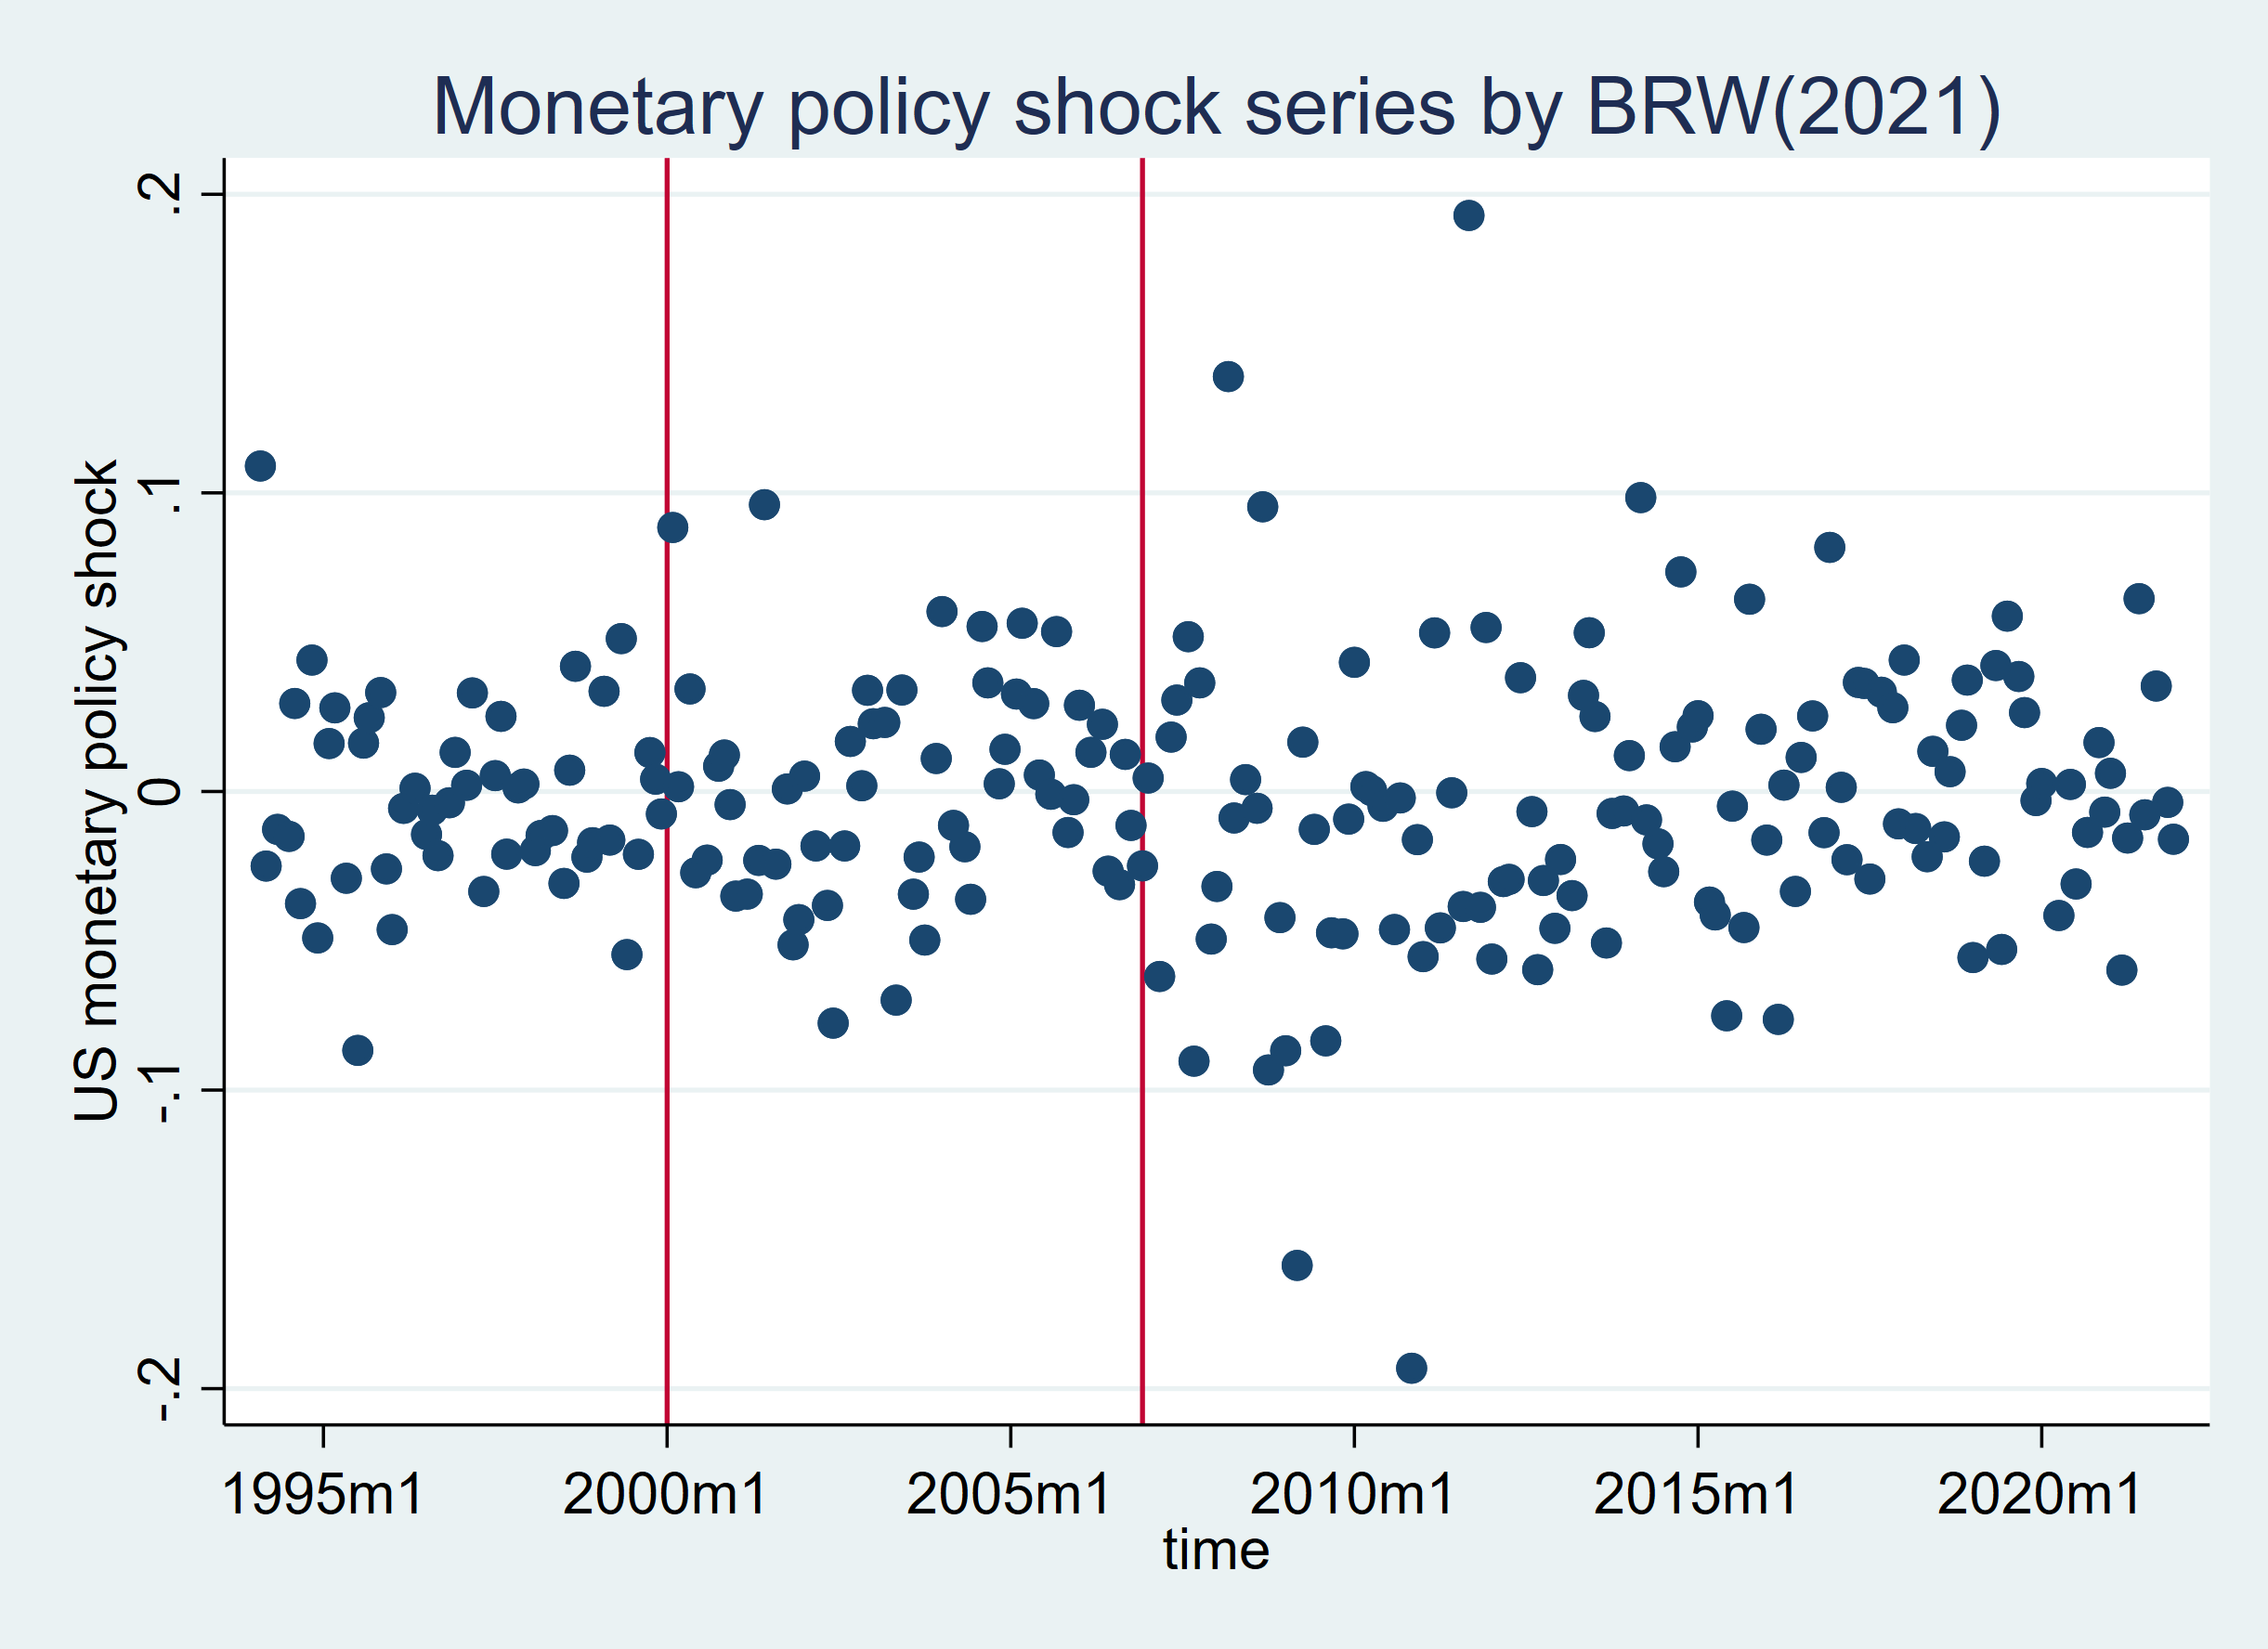
\includegraphics[width=\textwidth]{latex/drafts/pic/BRW.png}
    \caption{\small US monetary policy shock: \cite{bu2021unified}}
    \label{fig: BRW}
\end{figure}

\subsection{Customs trade data}

To investigate how exporters adjust their export prices in response to foreign monetary policy shocks, we merge the two disaggregated Chinese datasets: (1) the customs trade data between 2000 and 2006 and (2) the firm-level survey data.

We use the monthly transaction records from the General Administration of Customs of China (GACC). This dataset includes the most comprehensive information on all Chinese trade transactions, including each firm's import or export value denominated in US dollars, quantity, unit, product name and code, source or destination country, and the type of enterprises (e.g., state-owned, private, foreign-invested, and joint ventures), etc. In the raw data, each unique transaction refers to a firm-product-country-year entry. Of all customs information, each transaction's export value and quantity are of special interest because we can calculate the unit value by dividing the value by the quantity as an approximate measure of the export price, referring to the method of \cite{deloecker2012markups}. 

The categories of products in China's customs trade data are coded according to the Harmonized Coding and Description System (HS) of the World Customs Organization (WCO). The original data are subject to HS 8-digit classification. Since there were two major revisions of the HS system in 2002 and 2007, we aggregated HS8 product-level information to the HS6 level and then used conversion tables from the United Nations Trade Statistics to convert all codes into the older version of HS1996. We exclude unwanted observations referring to the standard of \cite{li2015exchange}: (1) products with inconsistent missing information of unit or quantity; (2) special product categories such as arms (HS2=93), antiques (HS2=97), and special categories (HS2=98 and 99); (3) transactions existing for only one year without any change over time.

Since we focus on the short-term price response of Chinese exporters, we use the disaggregated monthly-level records to match high-frequency monetary policy shocks, which is a major difference between this article and previous literature using Chinese customs data. To avoid including too much noise variation, we sum the price data to the firm level in the benchmark regressions; however, we can still exploit product and market differences if needed.

\subsection{Chinese firm-level data}

The source of Chinese firm-level production and financial information is the Annual Surveys of Industrial Enterprises in China (ASIE) conducted by the National Bureau of Statistics of China (NBSC). This database includes all state-owned enterprises and above-scale firms with more than 5 million RMB in annual sales. Between 2000 and 2006, the dataset records 160,000 in 2000 to 300,000. Previous studies of the Chinese economy have widely used this database since it contains details about firms’ identification codes, ownership, industry type, and about 80 other accounting variables on the three major accounting statements (i.e., balance sheets, profit \& loss accounts, and cash flow statements). Among all that information, our research will focus on the variables related to two aspects: (1) firms' production costs and sales, including total wage payment, total operation inputs, and sales income, etc., and (2) firms' financial costs and liquidity conditions, including financial expense and interest payment, total and net working capital, cash holding, and others.

Manufacturing firms participating in international trade in the matched sample are uniquely identified by each observation's FRDM (legal entity) code and the survey year. To deal with reporting errors in the ASIE, we drop unsatisfactory observations referring to the criteria of \cite{fan2015credit} and \cite{brooks2021agglomeration}. We only keep firms that satisfy the following conditions: (1) a firm’s identification number cannot be missing and must be unique; (2) the key financial variables (such as total assets and sales income) cannot be missing;  (3) the total assets must be higher than the liquid assets and the total fixed assets; (4) the total assets must be higher than the liquid assets and the fixed assets; (5) the sales income cannot be negative; (6) the total liability cannot be negative; (7) the number of employees hired by a firm must not be less than 10.

We follow the standard procedure to match the identification codes based on the firms' contact information as in \cite{feenstra2014exports} to merge these firm-level survey data with customs trade data. In Table \ref{tab.summary}, we provide summary statistics for firms' information and their export patterns in our matched sample. One notable point is that the distribution of firms' export value is skewed to the right long tail shape, with a few large exporters accounting for most of the trade value.

\begin{table}[htbp]
    \centering
    \caption{Summary statistics}
    \begin{threeparttable}
        \begin{tabular}{lccccc}
        \toprule
                &        Mean&          SD&         p50&         p25&         p75\\
        \midrule
        $\Delta P$        &        0.03&        0.42&        0.01&       -0.11&        0.17\\
        \# HS6 Products           &    6.29&       10.31&        3.00&        2.00&        7.00\\
        Export Value (*1000 USD)    &   76024&  8585801&     2437&      459&    10335\\
        Sales (*1000 RMB)   &   160148&  1201262&    34910&    15350&    90852\\
        Employment     &      449&     1210&      197&       96&      418\\
        $Debt$              &        0.55&        0.26&        0.56&        0.37&        0.74\\
        $IE/L$               &        0.02&        0.04&        0.01&        0.00&        0.03\\
        $Liquid$       &        0.10 &        0.29 &        0.10 &       -0.07 &        0.28\\
        $\phi^{exp}$ (Export/Sales)         &        0.46&        0.38&        0.36&        0.07&        0.89\\
        $\phi^{imp}$ (Import/Inputs)               &        0.18&        0.30&        0.01&        0.00&        0.25\\
        \midrule
        Firm-year observations        &     \multicolumn{5}{c}{270271}      \\
        \bottomrule
        \end{tabular}
        \begin{tablenotes}
    	\footnotesize
            \item Notes: This table shows the summary statistics of firms in the matched sample. The first row $\Delta P$ indicates monthly price changes, while all other rows describe annual-level firm variables. $Debt$ denotes the ratio of total liability over total assets, $IE/L$ denotes the ratio of interest expense over total liability, and $Liquid$ denotes the ratio of net liquid assets over total assets.
        \end{tablenotes}
    \end{threeparttable}
    \label{tab.summary}
\end{table}

\subsection{Export price index}

The customs dataset contains disaggregated trade values denominated by US dollars and quantities for each HS6 product $h$, each firm $i$, to each country $c$, at time $t$, $V_{ihct}$, and $Q_{ihct}$. We compute the unit values as the proxy of export prices:

$$
P_{ihct}=\frac{V_{ihct}}{Q_{ihct}}
$$

\noindent Because product categories are highly subdivided, we believe that the unit value is an ideal proxy for the transaction-level price. \footnote{In robustness checks, we also use the exchange rate between the US dollar and Chinese RMB to convert all trade values into RMB denominations, that is, we compute $P^{RMB}_{ihct}=\frac{V_{ihct} \cdot NER_{US,t}}{Q_{ihct}}$ where $NER_{US,t}$ is the bilateral nominal exchange rate of US dollars in terms of RMB in month $t$.}

Using the above unit value price, we construct a firm-level Tornqvist price index using detailed information about the price of each product in each destination market following \cite{smeets2013estimating}. First, we aggregate the unit value to the firm-product level, which is the average price of product $h$ produced by firm $i$ weighted by the relative sales to each market $c$ at time $t$, $P_{iht}=\sum_c s_{c,iht} P_{ihct}$, where the market-specific value share is $s_{c,ihct}=V_{ihct}/V_{iht}$. 

Second, we calculate the weighted average of the firm-product level price growth rate $\Delta_n \ln P_{iht} = \ln P_{iht}- \ln P_{ih(t-n)}$, for all product categories across $n$ periods: 

$$
\Delta_n \ln P_{it} = \sum _{h} \frac{s_{h,i(t-n)}+s_{h,it}}{2} \Delta_n \ln P_{iht}
$$

\noindent where the product-specific value share is $s_{h,it}=V_{iht}/V_{it}$, and the effective weight is the average value of product weights at time $t$ and $t-n$. In the baseline monthly price regression, we set the time gap $n$ as 12 months (one year). This firm-level price growth rate $\Delta_{12m} P_{it}$ describes year-over-year changes for the average export price of a certain exporter, considering all adjustments to both product and market scopes. We will exclude observations with the annual growth rate of unit value in the top or bottom one percentile to avoid results being affected by extreme idiosyncratic factors other than monetary policy shocks.

\newpage
\section{Empirical Results}

Our primary interest is to study the impacts of monetary policy shocks on export prices. This section describes our empirical specifications and shows how Chinese export prices adjust in response to unexpected US monetary policy shocks. We start from the baseline estimations of firm-level price response and then conduct robustness tests.

\subsection{Benchmark specification}

In our benchmark empirical analysis, we aggregate Chinese export prices at the firm level and treat this as our starting point. Although export unit values are at the firm-product-country level (namely, the transaction level), aggregation to firm-level price could avoid noises originating from too many dimensions. Besides global monetary policy shocks, we also add firm-fixed effect and other time-varying firm-level variables in the benchmark regression to control the firm-specific factors. Specifically, we :

\begin{equation}
    \Delta \ln P_{it} = \alpha+\beta \cdot m_{t}+ \Gamma \cdot \textbf{Z}_{it-n}+\xi_{i}+\varepsilon_{it}
\end{equation}

\noindent where $\Delta \ln P_{it}$ represents the year-over-year export price change of firm $i$ at time $t$ (compared with the same month in last year), $m_t$ represents the unexpected monetary policy shock at time $t$. In the baseline regression, we use the measure by \cite{bu2021unified} as our monetary policy shocks $m_t$, while alternative measures will also be employed in the robustness checks. Our variable of interest, $\beta$, represents the average price response to the concurrent monetary policy surprises. One advantage of using our exogenous monetary policy shock measure and micro-level price is to deliver causality directly. $\textbf{Z}_{it-n}$ denotes lagged controls of firm-level time-variant variables. The two most important control variables are price changes in the previous period (controlling for price adjustment autocorrelation) and real sales income in the previous year (controlling for firm size). To control for unobserved firm heterogeneity, we include $\xi_{i}$, the firm-level fixed effects that capture any time-invariant factors for a given firm.

\subsection{Export price responses to monetary policy shocks}

The baseline results are displayed in Figure \ref{fig.US_shock} and Table \ref{tab.baseline}: Chinese exporters will increase (decrease) their average prices in the short run, facing an unexpected contractionary (expansionary) US monetary policy shock. 

\begin{figure}[htbp]
    \centering
    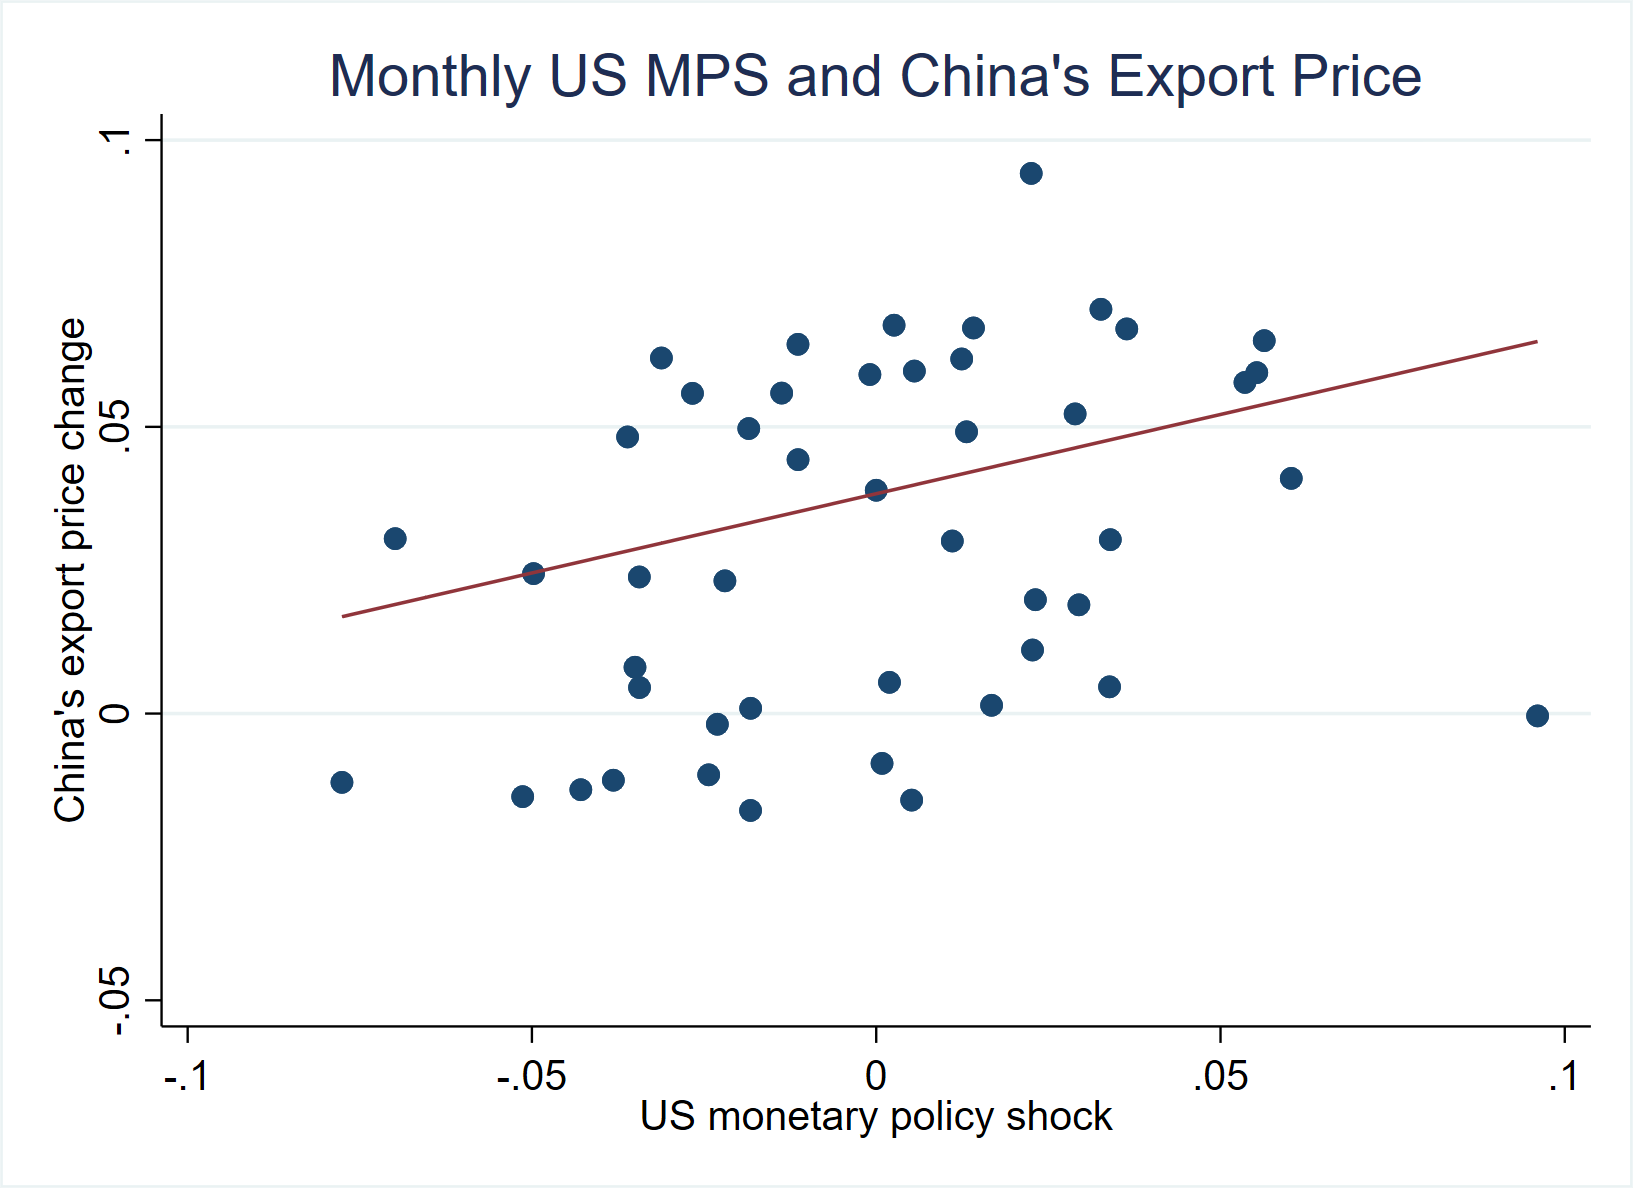
\includegraphics[width=0.8\columnwidth]{latex/slides/pic_Dec2023/brw_monthly.png}
    \caption{Monthly US monetary policy shocks and China's average export price}
    \label{fig.US_shock}
\end{figure}

In column (1) of Table \ref{tab.baseline}, we only include the monthly shock without other time-variant controls. We find that one unit of US monetary policy shock (100 basis point unexpected increase in the 2-year US treasury yield rate) will induce an 18 $\%$ monthly increase in China's export prions by average. From columns (2)-(3), we observe that controlling other firm-level factors slightly reduces the magnitude of the price response to around 14 $\%$, but the results are still significant. Columns (4)-(6) show the results when we aggregate the monthly sample to the annual level. In the annual sample, the dependent variable becomes annual price changes, and the monetary shock represents the sum of all the monthly shocks in that year. It turns out that the impact of the monetary shock is largely consistent with that of monthly regression.\footnote{As for the controlled variables, the coefficients are almost the opposite in the two versions; price changes display inertia in the short term and a pattern of mean regression in a relatively longer run, which is consistent with our intuition. Also, a firm with a bigger size tends to decrease its price in the short run while increasing the price in the longer run, which may be explained by the firm's price strategy and its market power. In this paper, we focus on the impact of global monetary policy shocks, so we will not explore this point in detail.} To summarize, we can observe a significant positive impact of unanticipated monetary policy shocks on export price movements: prices move in the same direction as interest rates. That is, a tighter monetary policy condition implies higher export prices.

    \begin{table}[htbp]
        \label{tab.baseline}
        \centering
        \caption{Export price responses to US monetary policy shocks}
        \resizebox{\columnwidth}{!}{
        \begin{threeparttable}
        \begin{tabular}{lcccccccc}
            \toprule
            & (1)   & (2)   & (3)   & (4)   & (5)   & (6) & (7)   & (8)\\
            & \multicolumn{4}{c}{Monthly $\Delta ln P_{it}$} & \multicolumn{4}{c}{Annual $\Delta ln P_{it}$}  \\
            \midrule
            $brw_t$   & 0.180*** & 0.182*** & 0.147*** & 0.150*** & 0.177*** & 0.189*** & 0.235*** & 0.244*** \\
                & (0.011) & (0.011) & (0.010) & (0.010) & (0.007) & (0.007) & (0.010) & (0.010) \\
            $Sales_{it-n}$ &     & -0.004** &       & -0.005*** &       & -0.017*** &       & -0.015*** \\
                  &   & (0.002) &       & (0.001) &       & (0.002) &       & (0.003) \\
            $\Delta ln P_{it-1}$ &    & & 0.301*** & 0.299*** &       & & -0.304*** & -0.303***  \\
                  &   &    & (0.003) & (0.003) &    &   & (0.005) & (0.005) \\
            $\Delta NER^{USD}_{t}$ & -0.777*** & -0.815*** & -0.610*** & -0.654*** & -0.717*** & -0.925*** & -0.976*** & -1.119*** \\
            & (0.048) & (0.051) & (0.036) & (0.039) & (0.046) & (0.052) & (0.061) & (0.066) \\
            \midrule
            Firm FE & Yes   & Yes   & Yes   & Yes   & Yes   & Yes & Yes   & Yes\\
            N     & 1100399 & 1072223 & 940015 & 917435 & 151542 & 147471 & 96296 & 96296 \\
            \bottomrule
            \end{tabular}
            \begin{tablenotes}
                \footnotesize
                \item Notes: Robust standard errors clustered at the firm level;  *, **, and *** indicate significance at 10\%, 5\%, and 1\% levels. The dependent variables in columns (1)-(4) are changes in monthly price, while columns (5)-(8) are changes in annual price. All regressions include firm fixed effects.
    	\end{tablenotes}
        \end{threeparttable}
        }
    \end{table}

There are two noteworthy aspects of these baseline results: (1) the coefficients describe the average level of price response for Chinese exports and do not contain information on the distribution of prices across firms, and (2) what is shown here is the significant effect of a monetary policy shock in the current period on prices over the period, which implies that at least a portion of the price changes immediately but does not rule out the possibility that long-run changes in prices may have been affected by multiple periods of monetary shocks. We also investigate the monthly dynamic responses and find that most of the adjustment takes place in the first six months, and the impact will gradually fade out within 12 months, indicating a short-term effect. The detailed results are displayed in Appendix \ref{tab.dynamic}.

\subsection{Robustness checks}

Our benchmark results are robust to many additional checks. First, we try \textit{alternative monetary policy shocks} in Table \ref{tab.altmps}. We first use the 30-minute high-frequency federal fund rate changes around the FOMC announcements to study the impact of conventional monetary policy shock, and then use the composite shock of \cite{nakamura2018high}, which is also a 30-minute high-frequency shock derived from the price changes of 2 federal fund rate futures and 3 Eurodollar futures around the FOMC announcement. This shock captures both the conventional monetary policy shock and the forward guidance. Moreover, we also employ the shock derived by \cite{guraynak2005actions}, who explicitly decompose an aggregate shock into the target and path part to represent conventional monetary policy shock and forward guidance, respectively, obtained from \cite{acosta2022perceived}. The shocks mentioned above may have the concern of information effect (see the literature like \cite{nakamura2018high}, \cite{jarocinski2020deconstructing}, \cite{acosta2022perceived}, etc.). Namely, the policy action of the Fed may signal its private information about current and future economic fundamentals. So we also test the impact of the pure monetary policy shock of \cite{jarocinski2020deconstructing} excluding any information shock using the co-movement of treasury yield and stock prices. All of these measures suggest that a tightening shock will move export prices upward.

\begin{table}[htbp]
    \centering
    \caption{Alternative monetary policy shocks}
    \resizebox{\columnwidth}{!}{
    \begin{threeparttable}
    \begin{tabular}{lcccccccc}
        \toprule
        & (1)   & (2)   & (3)   & (4)   & (5)   & (6) & (7)   & (8) \\
        & \multicolumn{2}{c}{$\Delta$ FFR} & \multicolumn{2}{c}{Nakamura \& Steinsson}  & \multicolumn{2}{c}{Acosta} & \multicolumn{2}{c}{Jarocinski \& Karadi}\\
        \midrule
        $\Delta FFR_t$ & 0.029*** & 0.025***&       &        &       &       &       &  \\
              & (0.008) & (0.007)&       &        &       &       &       &  \\
        $NS_t$  &       &    & 0.152*** & 0.144***     &       &  \\
              &       &   & (0.009) & (0.009)       &       &  \\
        $Target^{US}_t$ &       &       &       &       & 0.002*** & 0.002*** &       &  \\
              &       &       &       &       & (0.000) & (0.000) &       &  \\
        $Path^{US}_t$  &       &       &       &       & 0.005*** & 0.004*** &       &  \\
              &       &       &       &       & (0.000) & (0.000) &       &  \\
        $MP_t$ &       &       &       &       &       &       & 0.045*** & 0.068*** \\
              &       &       &       &       &       &       & (0.006) & (0.006) \\
        $\Delta ln P_{it-1}$ &       & 0.299*** &       & 0.300*** &       & 0.299*** &       & 0.300*** \\
              &       & (0.003) &       & (0.003) &       & (0.003) &       & (0.003) \\
        $Sales_{it-1}$ &       & -0.005*** &       & -0.004*** &       & -0.005*** &       & -0.004*** \\
              &       & (0.001) &       & (0.001) &       & (0.001) &       & (0.001) \\
        \midrule
        Firm FE & Yes   & Yes   & Yes   & Yes   & Yes   & Yes   & Yes   & Yes \\
        N     & 1100399 & 917435 & 1100399 & 917435 & 1100399 & 917435 & 1100399 & 917435 \\
        \bottomrule
    \end{tabular}
        \begin{tablenotes}
            \footnotesize
            \item Notes: Robust standard errors clustered at the firm level;  *, **, and *** indicate significance at 10\%, 5\%, and 1\% levels. The dependent variables in all columns are changes in monthly price. Monetary policy shock measures in columns (1)-(2), (3)-(4), (5)-(6), (7)-(8) are from Fed fund rate changes, \cite{nakamura2018high}, \cite{acosta2022perceived}, and \cite{jarocinski2020deconstructing}, respectively. All regressions include firm fixed effects.
	\end{tablenotes}
    \end{threeparttable}
    }
    \label{tab.altmps}
\end{table}

Second, we adopt \textit{alternative aggregation levels of price index} as in Table \ref{tab.altagg}. Firm-level price index adjustments give us an initial idea about price elasticity regarding monetary policy shocks. Here, we further use more disaggregated firm-product level prices and firm-product-country level prices as supplements. In the firm-product-country level regression, each transaction-level price is narrowly defined as the unit value of a certain product produced by a certain firm selling to a certain market. We add additional controls $RER_{ct}$, the bilateral real exchange rate between Chinese RMB and currency in the country $c$, and $RGDP_{ct}$, the real GDP of the source country deflated to the constant price level, which proxies for market demand. All results in those aggregation levels are consistent. 

Third, we limit our regression to \textit{sub samples}. To start with, in Table \ref{tab.single}, we repeat our baseline regressions on firms exporting only a single HS6 product within a given month. This test excludes any product switching effect affecting the firm-level price index. Although the sample size for single-product firms is much smaller, we observe similar price responses to monetary policy shocks. What's more, we show that our results are common for firms with different ownerships (see \textcolor{red}{Table}) and are robust to different destinations (see \textcolor{red}{Table}).

Fourth, we use \textit{alternative standard error cluster levels and fixed effects}. Compared with our benchmark monthly regression, we also use a firm-year level (year-month level, or sector level) cluster of standard error, and include additional year fixed effect respectively, and the results are robust (see Table \ref{tab.altfe}).

Fifthly, we converted all export prices back to \textit{US dollars}. Due to data limitations, we do not have specific information on the invoice currency used by each exporting company, but we know through anecdotal evidence that during the period studied in this article (2000-2006), the vast majority of China's exports were denominated in RMB or US dollars. The results using U.S. dollar prices show that export price adjustments in response to monetary policy shocks are not sensitive to the invoicing currency (see Table \ref{tab.USD}).

Finally, although our monetary policy shocks are unexpected and largely unpredictable from previous information, which to some degrees alleviates the endogeneity problem originating from omitted variables, we still add more macro economic indicators of China, the US and the world, such as inflation rate, industrial production growth rate, VIX, commodity prices, etc., to control the impact of time-varying factors on export prices. It suggests that results are robust (see \textcolor{red}{Table}).


\newpage
\section{Mechanism}

In this section, we will explore the mechanism behind our benchmark findings. According to the classical textbook open economy macroeconomic models, a tightening US monetary policy will push up global interest rates and incentivize households to consume less and deposit more, thus driving the shrinking of the global demand and decreasing product prices, contrary to our previous outcomes. Actually, apart from the demand-side story, the US monetary policy will also affect China's export prices on the supply side through its impact on firms' liquidity conditions and borrowing costs. In the following parts, we propose two possible channels. First, if firms have binding credit constraints, the US unexpected tightening will deteriorate firms' liquidity conditions, and exporters are incentivized to raise prices to alleviate credit constraints. Furthermore, we find that the impact of the US monetary shock depends on firms' liquidity conditions and it is bigger conditional on tighter circumstances. This is what we call the liquidity channel. The second one is the borrowing cost channel. Even when firms are not directly affected by credit constraints (i.e. unbinding constraints), liquidity worsening will also motivate firms to rely more on external financing thus causing a higher average borrowing cost. To compensate for these cost increases, firms will accordingly raise their export prices. Also, we find that this impact is more pronounced if the borrowing cost is higher. To verify the cost-driven channel, we decompose export price changes following the method of \cite{deloecker2012markups}into two parts: (1) the mark-up changes and (2) marginal cost changes. We display that only the marginal costs respond to the outside monetary shocks. What's more, we further reveal that the marginal cost increase is mainly due to borrowing costs instead of other input costs, such as material costs, labor costs, and the cost of imported goods. Finally, the US unanticipated tightening may increase China's interest rates and then drive up firms' borrowing costs. We reveal that this impact is relatively weak and the borrowing cost increases are mainly due to firms' higher reliance on external financing. 



\subsection{Liquidity channel}

As is documented in the literature (see \cite{manova2012export}, \cite{manova2013credit}, \cite{manova2015firm}) the behaviors of exporters are shaped by credit constraints. More specifically, firms usually need to borrow from outside institutions (e.g. banks) to partially or totally finance their working capital, and borrowing needs should not exceed credit access, which indicates that exporting behaviors are affected by firms' credit conditions. For example, if a firm has very limited credit access from commercial banks, how many products it will produce depends on how much money it can borrow. Previous papers usually highlight the role of time-invariant and sector-specific credit constraints, which reflect the long-run borrowing conditions of an industry. Instead, this paper focuses on firms' short-run time-varying credit conditions which are affected by firms' liquidity states. Liquidity deterioration may require a firm to borrow more from external institutions, which in turn affects exporting behaviors. Then, there is a role for global monetary policy shocks to alter a firm's exporting decisions through the impact on liquidity conditions. For instance, global monetary tightening may aggravate an exporter's liquidity, and firms are motivated to raise prices to get more cash flow to alleviate the adverse impact of liquidity shortage. The detailed mechanism illustrations are displayed in the model part.

To verify our conjecture, the strategy is to check how firms' liquidity is affected by US monetary shock. If the liquidity conditions worsen after an unexpected tightening shock, then it is consistent with our assumption. To measure a firm's liquidity conditions we use two direct measures, the net liquidity asset ratio (liquidity asset minus current liability over total assets) and the cash ratio (cash holding over total assets). Lower values correspond to tighter liquidity. Furthermore, we also employ two indirect measures, the turnover ratio (sales over inventory) and the trade credit provision ratio (account receivable to total sales). If a firm's liquidity worsens, its turnover is expected to be lower and it should provide less trade credit to its trade partners. The specification is directly regressing annual liquidity change on monetary shock which is also aggregated at the annual level with the control of firm size and total debt ratio (see \textcolor{red}{Equation}). All the data on liquidity measures are obtained from the Annual Surveys of Industrial Enterprises in China (ASIE) conducted by the National Bureau of Statistics of China (NBSC) from 2000 to 2006. 

$$
\textcolor{red}{Specification}
$$

From \textcolor{red}{Table} we find that an unexpected US tightening shock will significantly deteriorate firms' liquidity (both the direct and indirect measures). As for why liquidity worsens, there are possible two reasons. To start with, the US tightening may reduce the trade credit provisions of foreign firms to Chinese exporters. Another possible explanation is that the tightening shock will shrink global demand and thus reduce the firm's operational cash flow from exporting. This is consistent with our previous finding that the US contractionary shock will reduce the firm's export quantities and values (see \textcolor{red}{Table}).

Moreover, we show that the impact of monetary shock depends on the ex-ante liquidity conditions and it is bigger under tighter liquidity, which further strengthens the mechanism through liquidity. This conclusion is drawn from incorporating the interaction term of monetary shock and previous liquidity conditions into the benchmark regression (the specification is displayed in \textcolor{red}{Equation}), to alleviate endogeneity concern we aggregate the variables at the sector level and use the value of last year. Also, to control some time-specific common factors that can affect liquidity and price simultaneously, we add the time-fixed effect. It is seen in \textcolor{red}{Table} that the interaction terms are significantly negative. 


$$
\textcolor{red}{Specification}
$$


\subsection{Borrowing cost channel}

Even if a firm has sufficient credit access and is immune from credit constraints, the liquidity worsening after a tightening shock may still affect its pricing through the borrowing cost channel. More specifically, after a surprising US tightening, the deterioration of liquidity forces a firm to borrow more from external financial institutions, which provide relatively more expensive credits, thus driving up the average borrowing cost. To offset the lift-up of cost, the exporter raises its export prices. 

To test this channel, we first check how borrowing cost responds to the US monetary shock by regressing the annual borrowing cost change on monetary shock. This specification is similar to that of liquidity channel verification and the only difference is the dependent variable. To measure the average borrowing cost, we use four measures: the ratio of interest rate expenditure over total debt, the ratio of interest rate expenditure over current debt, the ratio of financial expenses over total debt, and the ratio of financial over current debt. All the data on borrowing cost measures are also obtained from the Annual Surveys of Industrial Enterprises in China (ASIE) database. As is displayed in \textcolor{red}{Table}, we find that the firm's borrowing cost significantly increases in response to a US contractionary shock, which is coherent with our previous conjecture. Furthermore, by including the interaction term of monetary shock and ex-ante borrowing cost into the benchmark specification (see \textcolor{red}{Equation}), we also illustrate that this impact is bigger if a firm faces higher borrowing costs.


To further reinforce the cost-driven channel, we also decompose the export price into mark-up and marginal cost following the method proposed by \cite{deloecker2012markups} and find that only marginal cost responds significantly to the US monetary shock and the reaction of mark-up change are quite weak both economically and statistically. The results are displayed in \textcolor{red}{Table}. What's more, we test that among all the costs, only the borrowing cost responds substantially while the material input cost, the labor cost, and the cost associated with imported goods don't matter too much. These results are shown in \textcolor{red}{Table}.

Regarding why borrowing costs increase after a tightening shock, there may be another possible explanation: US tightening increases Chinese interest rates. To verify this possibility, we regress the overnight return of Chinese treasury bonds and corporate bonds price index on the US monetary policy shock, and the results turned out to be relatively weak and insignificant although the reaction direction is consistent (see \textcolor{red}{Table}). This implies that the average borrowing cost movement is mainly driven by the higher reliance on more expensive external financing rather than the increases in the borrowing rate itself. This is plausible as China has quite tight capital control and tightly independent monetary authority thus China's financial market is not tightly exposed to US monetary policy adjustments. Similar results are also documented in previous papers such as \cite{hausman2011global} and \cite{ho2018hot}, etc. This result is interesting as it suggests that exporter's financing conditions are affected by external monetary shock even though the Chinese financial market itself responds quite mildly.


\subsection{Further verification}

To verify the channels proposed above, we also conducted several additional tests. Firstly, comparing the responses of ordinary processing trade exporters. The responses of processing trade should be smaller as its liquidity conditions are less affected by external shocks. Secondly, we rule out the possibility of a global demand shift by comparing the reaction of differentiated goods response to that of homogenous goods. We show that homogenous goods also significantly respond to the US shock and suggest that the price increases to a tightening shock is not doing to a global demand shift from other countries to China. Thirdly, we argue that our channel is an additional way to affect export prices apart from the exchange rate pass-through channel. This conclusion is yielded from the results that the impacts of monetary shock are still significant even when we control the bilateral real exchange rate changes.


\subsubsection{Ordinary VS processing trade}

Some exporters may be registered as "processing trade. That is, a processing trader imports raw materials and intermediate inputs from a foreign firm for domestic processing and re-exports to the same firm as its customer. Processing trade contracts is more fixed than that of ordinary trade. Moreover, financial frictions could affect firms' choice between processing and ordinary trade, which is a choice of production technology and its position in global supply chains. Therefore, processing trade could also implicitly imply some firm characteristics related to its market power (\cite{manova2016firms}). Due to the sorting mechanism, firms participating in more processing trade usually have less borrowing needs and are less constrained by liquidity conditions. So, suppose the borrowing cost and liquidity channels hold. In that case, we expect that facing the same monetary policy shock, the price response for processing traders should be smaller than that of ordinary traders.

We provide evidence about the price response patterns for ordinary trade compared with processing trade in Table \ref{tab.process}. Columns (1)-(2) only include the sample of ordinary trade transactions. In columns (3)-(4), we instead show the results using only processing trade transactions. In columns (5)-(6), we use the processing trade intensity as the interaction term to study the difference between processing and ordinary trade. In practice, in the firm-product level sample, we create a processing trade dummy, which takes the value of 1 when a transaction belongs to processing trade and 0 when it belongs to ordinary trade \footnote{When aggregating to a firm-level sample, we compute the processing trade intensity as the average number of processing trade products weighted by the export value.}. All these results show that the impact of US shock on processing traders is much smaller than that of ordinary traders, which verifies our conjecture and further reinforces our proposed mechanisms. Anyway, ordinary trade firms account for more than 2/3 of the total observations in our sample. Therefore, the pricing patterns based on ordinary trade should dominate the overall Chinese trade.

\begin{table}[h]
    \centering
    \caption{Ordinary trade vs processing trade}
    \begin{threeparttable}
    \begin{tabular}{lcccccc}
        \toprule
        & (1)   & (2)   & (3)   & (4)   & (5)   & (6) \\
          & \multicolumn{2}{c}{Ordinary trade}  & \multicolumn{2}{c}{Processing trade} & \multicolumn{2}{c}{Comparison}\\
        \midrule
        $brw_t$   & 0.201*** & 0.186*** & 0.098*** & 0.065*** & 0.225*** & 0.185*** \\
              & (0.018) & (0.019) & (0.019) & (0.016) & (0.016) & (0.016) \\
        $brw_t \times process_{it}$ &       &       &       &       & -0.102*** & -0.085*** \\
              &       &       &       &       & (0.024) & (0.023) \\
        $\Delta ln P_{it-1}$ &       & 0.190*** &       & 0.473*** &       & 0.299*** \\
              &       & (0.003) &       & (0.005) &       & (0.003) \\
        $Sales_{it-1}$ &       & -0.004* &       & -0.009*** &       & -0.004*** \\
              &       & (0.002) &       & (0.002) &       & (0.001) \\
        Firm FE & Yes   & Yes   & Yes   & Yes   & Yes   & Yes \\
        N     & 499418 & 391336 & 283952 & 242587 & 1100399 & 917435 \\
        \bottomrule
    \end{tabular}
        \begin{tablenotes}
            \footnotesize
            \item Notes: Robust standard errors clustered at the firm level;  *, **, and *** indicate significance at 10\%, 5\%, and 1\% levels. The dependent variables in columns (1)-(3) are changes in monthly price denominated in the US dollar, while columns (4)-(6) are changes in annual price denominated in the US dollar. All regressions include firm fixed effects.
	\end{tablenotes}
    \end{threeparttable}
    \label{tab.process}
\end{table}

\subsubsection{Homogeneous vs differentiated good}

In addition to the channels mentioned above, there might be two other potential explanations for the export price increase after a tightening US monetary shock:

(1) \textbf{Global demand shift} 

A tightening global monetary shock will induce a recession in a business cycle, which might make Chinese exports more competitive because some Chinese products are cheaper and of lower quality than similar ones from other developed countries. The idea is similar to the concept of Giffen goods: the prices of inferior goods increase when people's incomes drop. However, in Table \ref{tab.rauch}, we find that the prices of homogeneous goods also increase even more. These goods have little differences in quality and can't be treated as Giffen products. So, the mechanism shouldn't be attributed to a global demand shift.

\begin{table}[htbp]
    \centering
    \caption{Homogeneous good vs differentiated good}
    \resizebox{\columnwidth}{!}{
    \begin{threeparttable}
    \begin{tabular}{lcccccccc}
        \toprule
        & (1)   & (2)   & (3)   & (4)   & (5)   & (6)   & (7)   & (8) \\
        & \multicolumn{4}{c}{Conservative classification} & \multicolumn{4}{c}{Liberal classification} \\
        \midrule
        $brw_t$   & 0.170*** & 0.126*** & 0.149*** & 0.114*** & 0.168*** & 0.124*** & 0.148*** & 0.115*** \\
          & (0.011) & (0.011) & (0.012) & (0.012) & (0.012) & (0.011) & (0.013) & (0.012) \\
        $brw_t \times ToE_{it} $ & 0.152 & 0.112 &       &    & 0.263*** & 0.242***    &       &  \\
          & (0.128) & (0.125) &       &      & (0.086) & (0.082)     &       &  \\
        $brw_t \times Ref_{it} $ &       &       & 0.208*** & 0.125*** &       &    & 0.167*** & 0.082*** \\
          &       &       & (0.033) & (0.032) &       &         & (0.031) & (0.030)\\
        $\Delta ln P_{it-1}$ &       & 0.298*** &       & 0.298*** &       & 0.298*** &       & 0.298*** \\
          &       & (0.003) &       & (0.003) &       & (0.003) &       & (0.003) \\
        $Sales_{it-1}$ &       & 0.004*** &       & 0.004*** &       & 0.004*** &       & 0.004*** \\
          &       & (0.001) &       & (0.001) &       & (0.001) &       & (0.001) \\
    \midrule
    Firm FE & Yes   & Yes   & Yes   & Yes   & Yes   & Yes   & Yes   & Yes \\
    N     & 1014106 & 850174 & 1014106 & 850174 & 1014106 & 850174 & 1014106 & 850174 \\
        \bottomrule
    \end{tabular}
        \begin{tablenotes}
            \footnotesize
            \item Notes: Robust standard errors clustered at the firm level;  *, **, and *** indicate significance at 10\%, 5\%, and 1\% levels. The variables "ToE" and "Ref" represent the value share of goods traded on an organized exchange and the value share of reference-priced goods of firm $i$. Columns (1)-(4) use the "conservative" classification, while columns (5)-(8) use the "liberal" classification, both referring to \cite{rauch1999networks}. All regressions include firm fixed effects.
	\end{tablenotes}
    \end{threeparttable}
    }
    \label{tab.rauch}
\end{table}

\subsubsection{Exchange rate pass-through}
 
Classical monetary and exchange rate literature suggests that a tightening US monetary shock will cause the depreciation of the currencies in other countries. Moreover, many exchange-rate pass-through papers have revealed that exchange-rate depreciation will increase export prices denominated in domestic currency. However, this explanation is not likely to be the main reason for the price response. In most of our sample period, China's exchange rate regime is fixed to the US dollar; a US tightening shock will cause the RMB to appreciate against other currencies, so this story means the RMB-denominated price will follow the US dollar-denominated price. In addition, we have controlled the change of bilateral real exchange rate in the annual firm-product-country level regression (Columns (4)-(6) of Table \ref{tab.altagg}), and our results are robust. Finally, the average export exchange rate pass-through of Chinese firms is near complete (about 95\%), as in the related literature (\cite{li2015exchange}).

 
\newpage
\section{More Discussion}

\subsection{EU monetary policy shocks}

The European Central Bank (ECB) is another major central bank that can affect global financial conditions. Besides the spillover effect of US monetary policy shock, recent literature (see \cite{ca2020monetary}, \cite{corsetti2021exchange} and \cite{miranda2022tale}, etc.) indicates that the monetary policy of the European Central Bank (ECB) also has a substantial effect on global financial conditions and real economic activities. Using the same specification as our benchmark regression, we explore how China's export prices respond to the ECB monetary shocks in Table \ref{tab.EU}. In Column (1)-(3), we use the target shock from \cite{miranda2022tale} \footnote{Using the approach of \cite{swanson2021measuring}, \cite{miranda2022tale} decomposes the ECB monetary shock into three components: the target, path and lsap part, which reflects unexpected policy rate change, forward guidance and Large-scale asset purchasing respectively. In our main sample (2000-2006), traditional monetary policy dominates, so here, we only use the target shock.}. To avoid the confounding effect stemming from the central bank information effect, we also use the pure monetary policy shock of \cite{jarocinski2020deconstructing} in Column (4)-(6). It is seen that, unlike the reaction to the US shock, Chinese export prices barely move in response to the European monetary policy shocks. One unit of tightening target shock (increase 1-month OIS rate by 100 basis points) will decrease China's export prices by only 0.1$\%$ (see Column (3)). Also, when we use the pure monetary policy shock of \cite{jarocinski2020deconstructing}, this impact even becomes insignificant (see Column (6)). Our finding is consistent with the conclusion in the literature (like \cite{ca2020monetary}, \cite{corsetti2021exchange} and \cite{miranda2022tale}, etc.) that the spillover effect of ECB shock is less powerful than that of the Fed. This is easy to understand because the dominant role of the US dollar, along with the intensive integration of the global financial market, confers the US monetary policy with a special role in driving the global financial cycle (GFC) (\cite{miranda2020us}). Another possible explanation is that, in most of our sample period, China's exchange rate is fixed to the US dollar, and a substantial proportion of the transactions may invoiced in the US dollar, which may augment the impact of US shock on China's export prices. 

\begin{table}[htbp]
    \centering
    \caption{Export price responses to EU monetary policy shocks}
    \begin{threeparttable}
    \begin{tabular}{lcccccc}
        \toprule
        & (1)   & (2)   & (3)   & (4)   & (5)   & (6) \\
        & \multicolumn{3}{c}{Miranda-Agrippino \& Nenova} & \multicolumn{3}{c}{Jarocinski \& Karadi}  \\
        \midrule
        $m^{EU}_t$ & -0.002*** & -0.001*** & -0.001*** & -0.050*** & 0.002 & -0.002 \\
              & (0.000) & (0.000) & (0.000) & (0.011) & (0.011) & (0.011)\\  
        $\Delta ln P_{it-1}$ &       & 0.301*** & 0.300*** &       & 0.301*** & 0.300*** \\
              &       & (0.003) & (0.003) &       & (0.005) & (0.005) \\
        $Sales_{it-1}$ &       &       & -0.004*** &       &       & -0.004*** \\
              &       &       & (0.001) &       &       & (0.001) \\
        \midrule
        Firm FE & Yes   & Yes   & Yes   & Yes   & Yes   & Yes \\
         N     & 1100399 & 940015 & 917435 & 1100399 & 940015 & 917435 \\
        \bottomrule
    \end{tabular}
    \begin{tablenotes}
        \footnotesize
        \item Notes: Robust standard errors clustered at the firm level;  *, **, and *** indicate significance at 10\%, 5\%, and 1\% levels. Monetary policy shocks here are from the European Central Bank. The shock in columns (1)-(3) are obtained from \cite{miranda2022tale}, while columns (4)-(6) are  from \cite{jarocinski2020deconstructing}. All regressions include firm fixed effects.
    \end{tablenotes}
    \end{threeparttable}
    \label{tab.EU}
\end{table}

\subsection{Exchange rate regime shift: fixed VS floating}

Our monthly sample period covers 84 months from January 2000 to December 2006, when the RMB was pegged to the US dollar before July 2005. After that, China began to target a basket of currencies, allowing the fluctuation of the exchange rate to the US dollar. To investigate whether the export responses to global monetary shocks vary across exchange rate regimes, we split the whole sample into two parts: the fixed regime (Jan 2000 - June 2005) and the floating regime (July 2005 - Dec 2006) and redo the benchmark regression separately over the two sub-samples. In Table \ref{tab.regime}, we can see that the coefficient in the fixed regime is around 0.14 (Column 3), while it drops to 0.08 in the floating regime (Column 6). This indicates that the floating exchange serves as a buffer to external monetary shocks, but the spillover effect is not absolutely isolated, which is consistent with the conclusion in the literature, like \cite{shambaugh2004effect}, \cite{klein2012exchange}, \cite{georgiadis2016determinants}, \cite{dedola2017if}, etc. Therefore, the policy implication is that a more floating and flexible exchange rate regime can be adopted to mitigate the adverse impact of foreign monetary policy shocks.

\begin{table}[htbp]
    \centering
    \caption{Exchange rate regime shift: before and after July 2005}
    \begin{threeparttable}
    \begin{tabular}{lcccccc}
        \toprule
        & (1)   & (2)   & (3)   & (4)   & (5)   & (6) \\
        & \multicolumn{3}{c}{Fixed regime: before July 2005} & \multicolumn{3}{c}{Floating regime: after July 2005}  \\
        \midrule
        $brw_t$   & 0.189*** & 0.138*** & 0.138*** & 0.031 & 0.108*** & 0.080*** \\
              & (0.012) & (0.012) & (0.012) & (0.022) & (0.023) & (0.023) \\
        $\Delta ln P_{it-1}$ &       & 0.288*** & 0.287*** &       & 0.186*** & 0.182*** \\
              &       & (0.003) & (0.003) &       & (0.004) & (0.004) \\
        $Sales_{it-1}$ &       &       & 0.000 &       &       & -0.025*** \\
              &       &       & (0.002) &       &       & (0.004) \\
        \midrule
        Firm FE & Yes   & Yes   & Yes   & Yes   & Yes   & Yes \\
        N     & 708254 & 609726 & 594891 & 389776 & 328076 & 320432 \\
        \bottomrule
    \end{tabular}
        \begin{tablenotes}
            \footnotesize
            \item Notes: Robust standard errors clustered at the firm level;  *, **, and *** indicate significance at 10\%, 5\%, and 1\% levels. Columns (1)-(3) cover the period from January 2000 to July 2005, while columns (4)-(6) cover the period from August 2005 to December 2006. All regressions include firm fixed effects.
	\end{tablenotes}
    \end{threeparttable}
    \label{tab.regime}
\end{table}

\subsection{Asymmetric impact}









\newpage
\section{Model}

In this section, we construct a partial equilibrium model to show how exporting firms' behaviors respond to a global monetary contraction, which illustrates the mechanism is related to borrowing cost increases and liquidity constraints.  \footnote{A general equilibrium model will not alter the direction of the impact of global monetary policy shocks.} The model builds on the heterogeneous-firm trade model of \cite{melitz2003impact} and \cite{manova2013credit}, and we further incorporate the global monetary shocks. The main difference between the existing literature on firm credit constraints and trade is that, in this paper, the constraints are affected by global monetary shocks. The big picture is that a tightening global monetary shock will increase the borrowing cost and incentivize the firm to uplift its export price. Moreover, the contractionary shock worsens the firm's liquidity conditions, motivating it to increase prices to alleviate liquidity constraints.

\subsection{Benchmark model}

\textbf{Preferences and demand}

Although we only discuss the price expenses of Chinese exporters in the empirical part, we here introduce a more general trade model setting. The source and destination countries are denoted by $i$ and $j$, respectively. In this paper, $i$ is China, and $j$ denotes the rest of the world. Consumers in country $j$ can access a set of goods $X_j$, potentially different across countries. It is assumed that a representative consumer in country $j$ has a constant-elasticity-of-substitution (CES) utility function given by

\begin{equation}
U_j=(\int_{\omega \in \Omega_j} [\chi_{ij}(\omega)]^{\frac{\sigma-1}{\sigma}} d\omega\ )^\frac{\sigma}{\sigma-1}
\end{equation}

where $\chi_{ij}$ is country $j$’s quantity consumed of variety $\omega$ originated from country $i$, and $\sigma$ $>$ 1 is the elasticity of substitution between varieties. Therefore, consumer optimization yields the following demand function for variety $\omega$:

\begin{equation}
\chi_{ij}(\omega)=\frac{p_{ij}(\omega)^{-\sigma}}{P_j^{-\sigma}} Y_j
\end{equation}


where $p_{ij}(\omega)$ is the price of variety $\omega$, $P_j=(\int_{\omega \in \Omega_j} [p_{ij}(\omega)]^{1-\sigma} d \omega)^{\frac{1}{1-\sigma}}$ is an aggregate price index in country $j$, and $Y_j$ represents the total expenditure of country $j$. We assume that it is affected by global monetary shocks $m$ (e.g., US monetary shock): $Y_j=\bar{Y_j}+\rho_{Y}^j m+\epsilon_Y$, where $\bar{Y_j}$ is a trend component of $Y_j$, $\rho_{Y}^j<0$, $\epsilon_Y$ is a random error, and a positive $m$ means tightening shock. \footnote{Many papers have documented that US monetary policy tightening has a negative spillover effect on the GDP of other countries (e.g., \cite{kim2001international}, \cite{georgiadis2016determinants}, and \cite{iacoviello2019foreign}, etc.).} \\
 

\textbf{Exporting firm}

In each source country $i$, there is a continuum of firms that ex-ante differ in their productivity level $\phi_i$. We assume that there is only one input (e.g., materials or labor) for production, and the production function is $ y_i= \phi_i L_i$, where $\phi_i$ is productivity and $L_i$ is input. The firm in country $i$ minimizes its cost to satisfy the demand in the country $j$, $\chi_{ij}(\omega)=\frac{p_{ij}(\omega)^{-\sigma}}{P_j^{-\sigma}} Y_j$. This yields a total cost function $ C_{ij}=\frac{w_i}{\phi_i} \frac{p_{ij}(\omega)^{-\sigma}}{P_j^{-\sigma}} Y_j$, where $w_i$ is the price of input. To capture the demand side effect, we allow the input price to fluctuate in response to global monetary shocks: $w_i=\bar{w_i}+\rho_w^i m + \epsilon_w^i$, where $\bar{w_i}$ is a trend component of $w_i$, $\rho_w^i<0$ and $\epsilon_w^i$ is a random error.\footnote{According to the demand side story, a contractionary global monetary shock may depress domestic total demand, and hence decrease the demand of inputs and also their prices.} 

We further assume a working capital constraint that a fraction $\delta_i$ of the input costs should be borrowed from outside financial institutions (e.g., bank loans or issuing bonds) and paid in advance\footnote{Compared with domestic sales or purchasing, the cross-border exporting or importing is riskier and more demanding, and relying more on additional external capital(\cite{manova2013credit}).}. Here $\delta_i$ $\in$ [0, 1] and is a decreasing function of firm's liquidity condition and trade credit: $\delta_i \equiv 1-c_i^\gamma-\zeta_i$, where $c_i$ $\in$ [0, 1] and is the liquidity condition (bigger value means better situation), $\gamma$ is a positive constant and reflects the elasticity of borrowing fraction with respect to liquidity condition, $\zeta_i$ is the fraction of input costs that is supported by trade credit. \footnote{The intuition is that a firm with better liquidity conditions and trade credit has less need for external financing.} Here, $c_i$ is assumed to be impacted by monetary policy shock exogenously: $c_i=\bar{c_i}+\rho_c^i m+\epsilon_c^i$, where $\bar{c_i}$ is a trend component of $c_i$, $\rho_c^i<0$ and $\epsilon_c^i$ is a random error.\footnote{The cash flow from sales income and the balance sheet may be adversely affected after a contractionary shock. For simplicity, here, the liquidity conditions are assumed to be exogenous, and the endogenization of cash holding will not alter our main mechanisms.} Trade credit is also assumed to be affected by global monetary shocks: $\zeta_i=\bar{\zeta_i}+\rho_\zeta^i m+\epsilon_t^i$, where $\bar{t_i}$ is a trend component of $\zeta_i$, $\rho_\zeta^i<0$ and $\epsilon_\zeta^i$ is a random error. \footnote{\cite{lin2018foreign} revealed that global liquidity shocks may deteriorate domestic trade credit.} 

Thus the cost function becomes $ C_{ij}=\frac{w_i(1-\delta_i+\delta_i R_i)}{\phi_i} \frac{p_{ij}(\omega)^{-\sigma}}{P_j^{-\sigma}} Y_j$, where $R_i$ is the gross borrowing interest rate in country $i$. We explicitly assume $R_i=\bar{R_i}+\rho_R^i m+\epsilon_R^i$ where $\bar{R_i}$ is a trend component of $R_i$, $\rho_R^i>0$ and $\epsilon_R^i$ is a random error.\footnote{The literature (like \cite{georgiadis2016determinants} and \cite{miranda2020us}, etc.) has reached an agreement that the borrowing cost of domestic firms will increase after a contractionary global monetary policy shock. Here, we assume it is exogenous, and the firm takes it as given. The endogenization of borrowing costs will not change our main results.} Also, to allow the non-linear elasticity of cost with respect to interest rate (which can be generated by other financial costs associated with borrowing), we replace $R_i$ with $R_i^\alpha$, where $\alpha$ is a constant and represents the elasticity of cost with respect to the interest rate. Following the convention, we also add an iceberg trade cost such that $\tau_{ij}\geq1$ units of good must be shipped from country $i$ for one unit to arrive in $j$. For the simplicity of notation, the subscripts for source and destination and the index for variety are omitted. Thus, the new cost function is

\begin{equation}
C=\frac{\tau w(1-\delta+\delta R^\alpha)}{\phi} \frac{p^{-\sigma}}{P^{-\sigma}} Y
\end{equation}

We also assume that firms cannot borrow more than a fraction $\theta$ of the expected cash flow from exporting, and it is smaller when $R$ is higher. The intuition behind this is that higher interest rates imply higher risk, and access to credit should be lower. Without loss of generality, we can assume $\theta=R^{-\nu}$, where $\nu$ is $>0$ and reflects the elasticity of financial credit access with respect to the interest rate. The optimization problem of the firm is 

$$
\max_{p} \ (p- \frac{\tau w(1-\delta+\delta R^\alpha)}{\phi}) \frac{p^{-\sigma}}{P^{-\sigma}} Y
$$

\begin{equation}
\text{s.t.} \ \theta [(p-\zeta \frac{\tau w}{\phi}) \frac{p^{-\sigma}}{P^{-\sigma}} Y]\geq(1-c^\gamma-\zeta)\frac{\tau w}{\phi} \frac{p^{-\sigma}}{P^{-\sigma}} Y
\end{equation}


\textbf{Case 1: borrowing constraint is binding: }

If $\theta<=\bar{\theta}$, where $\bar{\theta}$ is a threshold, the borrowing constraint is binding and we can rewrite the borrowing constraint as 

\begin{equation}
p=[(1-R^{\nu})\zeta+(1-c^\gamma)R^{\nu}] \frac{\tau w}{\phi}
\end{equation}

\textbf{Case 2: borrowing constraint is not binding}

If $\theta>\bar{\theta}$, the borrowing constraint is not binding. Solving the unconstrained optimization problem will give us that

\begin{equation}
p=\frac{\sigma}{\sigma-1}\frac{\tau w [c^\gamma+\zeta+(1-c^\gamma-\zeta) R^\alpha]}{\phi}
\end{equation}

This reduces to $p=\frac{\sigma}{\sigma-1}\frac{\tau w}{\phi}$ if $c$=0 and $R$=1, which is similar to \cite{melitz2003impact} \\


\textbf{Proposition 1.} The export price increases with the borrowing rate and decreases with liquidity condition and trade credit: $\frac{\partial p}{\partial R}>0$, $\frac{\partial p}{\partial c}<0$ $\frac{\partial p}{\partial \zeta}<0$

\textit{Proof}

If the borrowing constraint is binding:
$$
\frac{\partial p}{\partial R}=\frac{\tau w}{\phi}(1-c^\gamma-\zeta)\nu R^{\nu-1}>0
$$
$$
\frac{\partial p}{\partial c}=\frac{\tau w}{\phi} R^\nu(-1)\gamma c^{\gamma-1}<0
$$
$$
\frac{\partial p}{\partial \zeta}=\frac{\tau w}{\phi}(1-R^\nu)<0
$$

If the borrowing constraint is not binding:
$$
\frac{\partial p}{\partial R}=\frac{\sigma}{\sigma-1}\frac{\tau w}{\phi}[\alpha(1-c^\gamma-\zeta)R^{\alpha-1}]>0
$$
$$
\frac{\partial p}{\partial c}=\frac{\sigma}{\sigma-1}\frac{\tau w}{\phi}\gamma(1-R^\alpha)c^{\gamma-1}<0
$$
$$
\frac{\partial p}{\partial \zeta}=\frac{\sigma}{\sigma-1}\frac{\tau w}{\phi} (1-R^\alpha)<0
$$


\textbf{Proposition 2.} The export price increases after a tightening shock (i.e. $\frac{\partial p}{\partial m}>0$) if the supply side effect dominates.

\textit{Proof}

If the borrowing constraint is binding:

\begin{align*} 
\frac{\partial p}{\partial m} =&\frac{\partial p}{\partial R}\frac{\partial R}{\partial m}+\frac{\partial p}{\partial c}\frac{\partial c}{\partial m}+\frac{\partial p}{\partial \zeta}\frac{\partial \zeta}{\partial m}+\frac{\partial p}{\partial w}\frac{\partial w}{\partial m}  \\
=& \frac{\tau w}{\phi}(1-c^\gamma-\zeta)\nu R^{\nu-1} \rho_R+ \frac{\tau w}{\phi} R^\nu(-1)\gamma c^{\gamma-1} \rho_c +\\  
& \frac{\tau w}{\phi}(1-R^\nu) \rho_t+\frac{\tau}{\phi}[(1-R^\nu)\zeta+(1-c^\gamma)R^\nu] \rho_w
\end{align*} 

If the borrowing constraint is not binding:

\begin{align*} 
\frac{\partial p}{\partial m} =&\frac{\partial p}{\partial R}\frac{\partial R}{\partial m}+\frac{\partial p}{\partial c}\frac{\partial c}{\partial m}+\frac{\partial p}{\partial \zeta}\frac{\partial \zeta}{\partial m}+\frac{\partial p}{\partial w}\frac{\partial w}{\partial m}  \\
=& \frac{\sigma}{\sigma-1}\frac{\tau w}{\phi}[\alpha(1-c^\gamma-\zeta)R^{\alpha-1}] \rho_R + \frac{\sigma}{\sigma-1}\frac{\tau w}{\phi}\gamma(1-R^\alpha)c^{\gamma-1} \rho_c + \\
& \frac{\sigma}{\sigma-1}\frac{\tau w}{\phi} (1-R^\alpha) \rho_\zeta + \frac{\sigma}{\sigma-1}\frac{\tau}{\phi}[c^\gamma+\zeta+(1-c^\gamma-\zeta)R^\alpha] \rho_w
\end{align*} 

In both cases, the first three parts $\frac{\partial p}{\partial R}\frac{\partial R}{\partial m}$, $\frac{\partial p}{\partial c}\frac{\partial c}{\partial m}$, $\frac{\partial p}{\partial \zeta}\frac{\partial \zeta}{\partial m}$ are positive, while the fourth part $\frac{\partial p}{\partial w}\frac{\partial w}{\partial m} $ is negative. The former three parts are related to the supply-side effect, and the last part reflects the power of demand shrink. When the supply-side cost-push effect dominates the demand effect, the net impact of global monetary policy shock should be positive. 

\textbf{Proposition 3.} The impact of monetary shock on export price (i.e. $\frac{\partial p}{\partial m}$) is non-linear. Conditional on the value of specific parameters, it is bigger when $R$ is larger and $c$ (or $\zeta$) is smaller.

\textit{Proof}

This can be easily derived from Proposition 2 as $\frac{\partial p}{\partial m}$ will be an increasing function of $R$ and a decreasing function of $c$ and $\zeta$ given some sets of parameters. The existence of this non-linearity could be verified empirically.





\newpage
\section{Conclusion}

In this paper, we have explored the response of export prices to global shocks, which is a fundamental aspect of international economics. Different from the existing literature, our focus is specifically on monetary policy shocks originating from the United States, which behaves as a pivotal force driving the global financial cycle. Using high-frequency exogenous monetary shocks, monthly custom transaction records, and comprehensive firm-level balance sheet data, we provide a fresh perspective on this subject. This paper documents a counter-intuitive finding that exporters do not lower their export prices in response to a contraction in total demand following a tightening of US monetary policy. Instead, the monetary contraction acts as a cost-push factor from the supply side, prompting exporters to raise their prices to offset the negative impact. Furthermore, we reveal tightening US monetary policy shock will deteriorate global liquidity conditions, and firms are incentivized to raise prices to alleviate their liquidity constraints. We also illustrate that the impact of US monetary policy shocks is non-linear and more pronounced for firms with higher borrowing costs and less favorable liquidity conditions.

In an era characterized by the increasing integration of global trade and finance, understanding how export prices adapt to global monetary policy shocks in the presence of financial frictions is crucial for both market players and policymakers. Our paper casts new light on the special role of US monetary policy shocks in shaping international trade through its influence on global financing cost and liquidity conditions. Using China, the biggest exporter in the world, as an example of general implications for all economies, especially those developing countries where exporters are usually financially constrained. Although our paper mainly focuses on the response of exporter behaviors, the finding may also provide enlightenment for some other research, such as the global monetary policy spillover on the real economy and asset prices through trade channels, the impact of international monetary shocks on global inflation in the presence of cross-border trade linkages, and the optimal domestic policy and international coordination in response to adverse global shocks in the presence of financial friction, etc. Many interesting and important questions have remained in this area, and we hope our paper serves as a stepping stone for future research.


\newpage
\bibliography{latex/setup/reference}

\appendix

\section{A. More results on benchmark regression}\label{app_benchmark}

\section{B. More results on mechanism}\label{app_mechanism}

\section{C. Model extension}\label{app_model}


Our conclusion in the benchmark model is robust to sticky price setting, currency invoicing, and fixed costs inclusion, which are illustrated below. \\

\textbf{Dynamic optimization and sticky price} \\

In the benchmark model, the optimization problem is static, and the prices are assumed to be flexible. In this part, we are going to illustrate that the main mechanisms still hold under dynamic optimization and sticky prices. We use the classical \cite{calvo1983staggered} sticky price setting, and the firm's problem is to maximize its expected real profits:

$$
\max_{p_t} \ \mathbb{E}_t \sum_{i=0}^{\infty} \lambda^i \Omega_{i,t+i} \biggr[ \frac{p_t}{P_{t+i}}-\frac{\tau_{t+i} w_{t+i}(1-\delta_{t+i}+\delta_{t+i} R_{t+i}^\alpha)}{\phi_{t+i}P_{t+i}} \biggr] \frac{p_t^{-\sigma}}{P_{t+i}^{-\sigma}}Y_{t+i}
$$

\begin{align*}
\text{s.t.} \ &\mathbb{E}_t \sum_{i=0}^{\infty} \lambda^i \Omega_{i,t+i} \frac{P_t}{P_{t+i}} \biggr[ \theta_{t+i} (p_t-\zeta_{t+i} \frac{\tau_{t+i} w_{t+i}}{\phi_{t+i}}) \frac{p_t^{-\sigma}}{P_{t+i}^{-\sigma}}Y_{t+i} \biggr] \geq  \\
 &\mathbb{E}_t \sum_{i=0}^{\infty} \lambda^i \Omega_{i,t+i} \frac{P_t}{P_{t+i}} \biggr[(1-c_{t+i}^{\gamma}-\zeta_{t+i}) \frac{\tau_{t+i} w_{t+i}}{\phi_{t+i}} \frac{p_t^{-\sigma}}{P_{t+i}^{-\sigma}}Y_{t+i}\biggr]    
\end{align*}

where $\Omega_{i,t+i}$ is the real stochastic discount factor, and $\lambda$ is the probability of a firm keeping its price unchanged in each period. The left-hand side of the borrowing constraint is the weighted sum of credit access, and the right-hand side reflects the corresponding external credit demands.

If the borrowing constraint is binding, we can rearrange the constraint and obtain the expression of the export price:

\begin{equation}
p_t=\frac{\sum_{i=0}^{\infty} \lambda^i \Omega_{i,t+i}\frac{Y_{t+i}}{P_{t+i}^{1-\sigma}}\frac{\tau_{t+i}w_{t+i}}{\phi_{t+i}}(R_{t+i}^{-\nu}\zeta_{t+i}+\delta_{t+i})}{\sum_{i=0}^{\infty} \lambda^i \Omega_{i,t+i}\frac{Y_{t+i}}{P_{t+i}^{1-\sigma}}R_{t+i}^{-\nu}}
\end{equation}

It is seen that a tightening monetary shock can raise prices by increasing the borrowing proportion $\delta_{t+i}$ and reducing the ratio of credit access $R_{t+i}^{-\nu}$. The channel is similar to the static problem we discussed before. However, in this case, the impact of the monetary shock on the aggregate expenditure $Y_{t+i}$ and price index $P_{t+i}$ will also play a role, which reflects the power of general equilibrium. If $\lambda=0$, $p=[(1-R^{\nu})\zeta+(1-c^\gamma)R^{\nu}] \frac{\tau w}{\phi}$, which is identical to the static solution.


If the borrowing constraint is not binding, we solve the unconstrained problem and get the first-order condition:


\begin{equation}
\mathbb{E}_t \sum_{i=0}^{\infty} \lambda^i \Omega_{i,t+i} \biggr[(1-\sigma)\frac{p_t}{P_{t+i}}+\sigma \varphi_{t+i}\biggr]\frac{1}{p_t}\frac{p_t^{-\sigma}}{P_{t+i}^{-\sigma}}Y_{t+i}=0
\end{equation}

Where $\varphi_{t+i}\equiv \frac{\tau_{t+i} w_{t+i}(1-\delta_{t+i}+\delta_{t+i} R_{t+i}^\alpha)}{\phi_{t+i}P_{t+i}}$ is the real marginal cost. The optimal price can be expressed as:

\begin{equation}
p_t=\frac{\sigma}{\sigma-1}\frac{\mathbb{E}_t \sum_{i=0}^{\infty} \lambda^i \Omega_{i,t+i}\frac{P_t^{-\sigma}}{P_{t+i}^{-\sigma}}Y_{t+i}\varphi_{t+i}}{\mathbb{E}_t \sum_{i=0}^{\infty} \lambda^i \Omega_{i,t+i}\frac{P_t^{-\sigma}}{P_{t+i}^{1-\sigma}}Y_{t+i}}
\end{equation}

We can see that a global monetary policy shock can still affect export prices through its impact on current and future real marginal costs $\phi_{t+i}$. More specifically, a tightening shock can increase the borrowing cost $R_{t+i}$ and the borrowing proportion $\delta_{t+i}$. The channel is similar to the static problem we discussed before, and now the impact is a weighted sum of the effect on current and future marginal costs. If $\lambda=0$, $p_t=\frac{\sigma}{\sigma-1}\frac{\tau_{t} w_{t}(1-\delta_{t}+\delta_{t} R_{t}^\alpha)}{\phi_{t}}$, which is exactly the same as the static version. \\


\textbf{Invoicing currency} \\

Our benchmark model doesn't explicitly consider the role of exchange rates and invoicing currency. In this part, we will explain that our mechanisms are robust to producer currency pricing (PCP), US Dollar currency pricing (DCP), and local currency pricing (LCP). 

\textbf{\textit{PCP}} The firm's problem is 

$$
\max_{p} \ (p- \frac{\tau w(1-\delta+\delta R^\alpha)}{\phi}) (\frac{p}{e_jP_j})^{-\sigma} Y_j
$$

$$
\text{s.t.} \ \theta [(p-\zeta \frac{\tau w}{\phi}) (\frac{p}{e_jP_j})^{-\sigma} Y]\geq(1-c^\gamma-\zeta)\frac{\tau w}{\phi} (\frac{p}{e_jP_j})^{-\sigma} Y_j
$$

where $p$ is the price in the producer currency, $e_j$ is the nominal exchange rate, defined as the price of the destination country $j$ currency in terms of the producer currency, $P_j$ is a price index in country $j$, and $Y_j$ is the total expenditure in country $j$.

If the constraint is binding
$$
p=[(1-R^{\nu})\zeta+(1-c^\gamma)R^{\nu}] \frac{\tau w}{\phi}
$$

If the constraint is not binding

$$
p=\frac{\sigma}{\sigma-1}\frac{\tau w [c^\gamma+\zeta+(1-c^\gamma-\zeta) R^\alpha]}{\phi}
$$

This is similar to our benchmark expression of optimal prices. \\

\textbf{\textit{DCP}} The firm's problem is   

$$
\max_{p} \ (pe_{us}- \frac{\tau w(1-\delta+\delta R^\alpha)}{\phi}) (\frac{pe_{us}}{e_jP_j})^{-\sigma} Y_j
$$

$$
\text{s.t.} \ \theta [(pe_{us}-\zeta \frac{\tau w}{\phi}) (\frac{pe_{us}}{e_jP_j})^{-\sigma} Y]\geq(1-c^\gamma-\zeta)\frac{\tau w}{\phi} (\frac{pe_{us}}{e_jP_j})^{-\sigma} Y_j
$$

where $p$ is the price in the US dollar, $e_{us}$ is the nominal exchange rate against the US, defined as the price of the US dollar in terms of the producer currency.

If the constraint is binding
$$
pe_{us}=[(1-R^{\nu})\zeta+(1-c^\gamma)R^{\nu}] \frac{\tau w}{\phi}
$$

If the constraint is not binding

$$
pe_{us}=\frac{\sigma}{\sigma-1}\frac{\tau w [c^\gamma+\zeta+(1-c^\gamma-\zeta) R^\alpha]}{\phi}
$$

The price in the producer currency $pe_{us}$ is similar to the benchmark solution. As for the price in the US dollar, if the exchange rate is floating, the impact of a tightening US monetary shock is smaller as the exchange rate will increase after a tightening US monetary shock.


\textbf{\textit{LCP}} The firm's problem is 

$$
\max_{p} \ (pe_j- \frac{\tau w(1-\delta+\delta R^\alpha)}{\phi}) (\frac{p}{P_j})^{-\sigma} Y_j
$$

$$
\text{s.t.} \ \theta [(pe_j-\zeta \frac{\tau w}{\phi}) (\frac{p}{P_j})^{-\sigma} Y]\geq(1-c^\gamma-\zeta)\frac{\tau w}{\phi} (\frac{p}{P_j})^{-\sigma} Y_j
$$


If the constraint is binding
$$
pe_{j}=[(1-R^{\nu})\zeta+(1-c^\gamma)R^{\nu}] \frac{\tau w}{\phi}
$$

If the constraint is not binding

$$
pe_{j}=\frac{\sigma}{\sigma-1}\frac{\tau w [c^\gamma+\zeta+(1-c^\gamma-\zeta) R^\alpha]}{\phi}
$$

Similarly, the price in the producer currency $pe_{j}$ is identical to the benchmark solution. As for the price in the local currency, the impact is also affected by the response of the exchange rate $e_j$. \\



\textbf{Both variable and fixed costs are paid in advance} \\

If we incorporate fixed costs into the benchmark model and allow a proportion of $\delta$ ($\equiv 1-c^{\gamma}-\zeta$) of both types of costs to be paid in advance. The firm's problem now becomes

$$
\max_{p} \ (p- \frac{\tau w(1-\delta+\delta R^\alpha)}{\phi}) \frac{p^{-\sigma}}{P^{-\sigma}} Y-f
$$

\begin{equation}
\text{s.t.} \ \theta [(p -\zeta \frac{\tau w}{\phi}) \frac{p^{-\sigma}}{P^{-\sigma}} Y -\zeta f ]\geq(1-c^\gamma-\zeta) (\frac{\tau w}{\phi} \frac{p^{-\sigma}}{P^{-\sigma}} Y+f)
\end{equation}

where $f$ is the fixed cost; if the constraint is not binding, the result is similar to the benchmark model result; if the constraint is binding, we can rewrite it as 

\begin{equation}\label{eq:constraint_fixedcost}
p^{1-\sigma}=[(\frac{1-c^{\gamma}-\zeta}{\theta}+\zeta)\frac{\tau w}{\phi}] (p^{1-\sigma})^{\frac{\sigma}{\sigma-1}}+f(\frac{1-c^{\gamma}-\zeta}{\theta}+\zeta)\frac{P^{-\sigma}}{Y}
\end{equation}

Adding the new constraint into the objective function, we get the profit: 

\begin{equation}
[\frac{1-c^\gamma-\zeta}{R^{-\nu}}-c^\gamma-(1-c^\gamma-\zeta)R^{\alpha}]\frac{\tau w}{\phi} \frac{p^{-\sigma}}{P^{-\sigma}}Y+f(\frac{1-c^\gamma-\zeta}{R^{-\nu}}-1+\zeta)
\end{equation}


To solve Equation \ref{eq:constraint_fixedcost}, we can illustrate it with Figure \ref{fig: fixed_cost}, the straight line represents the left-hand side, and the curve denotes the right-hand side. There are two intersections of these two lines, which means there are two solutions to this equation. Since the profit is a decreasing function of $p$, the firm will choose the lower price, corresponding to $p_H^{1-\sigma}$. When interest rate $R$ increases, liquidity condition $\zeta$ and trade credit $\zeta$ decreases, the curve moves upward, and $p_H^{1-\sigma}$ will be smaller, which yields a higher optimal price. So, Proposition 1 still holds. A tightening shock will drive up interest rates, deteriorate liquidity conditions, and decrease trade credit, so the price goes up. Namely, Proposition 2 also holds. Furthermore, given some sets of parameters, a one percent increase in $R$ and a decrease in $c$ and $\zeta$ will cause the curve to move upward with a bigger magnitude. Thus, one unit of monetary shock will induce a bigger price change. This is exactly in line with what Proposition 3 predicts. To sum up, including fixed costs will not alter our main propositions.

\begin{figure}[H]
     \centering
         
\includegraphics[width=0.9\textwidth]{latex/drafts/pic/fixed_cost.png}
         \caption{\small Borrowing constraint when both variable and fixed costs are paid in advance}
         \label{fig: fixed_cost}
\end{figure}

\end{document}